\chapter{Results and Discussion} \label{sec:discussion}
In the following, results from each model are documented and briefly compared. Then, an in-depth discussion on potential methods for optimising the models will take place. Finally, suggestions for further work in the research field will be made.

Two types of supervised problems were considered: regression and classification. Due to the fundamental difference in the output values of models for these two tasks (one decimal number per feature in the former, several binary class predictions per feature in the latter), in order to enable comparison between the models, the terms \textit{hit} and \textit{hit rate} were introduced.

For classification models, a hit is simply a correct label prediction. A hit by a regression model was defined as a damage prediction, \(y_\text{pred}\), accurate within a tolerance of \(\pm0.15\) cycles from the SA66 value, \(y_\text{true}\). The value of 0.15 is somewhat arbitrary and by no means an acceptable tolerance for a model in production, but is a sufficiently challenging but achievable goal for the current research stage and should therefore offer a suitable comparison. The hit rate (HR) is determined by dividing the number of hits by the total number of predictions.

The metrics used for describing regression models are \(R^2\) (described in Section \ref{sec:polyreg}) to measure the quality of the fit, and the feature-wise mean hit rate (MHR).

For the classification problem, metrics used are the hit rate per feature and the mean absolute error per feature. Since the class labels generated (as opposed to those predicted) are ordinal (see Section \ref{sec:data:classification_rep}), error for classification models was defined as the difference between \(Y_\text{pred}\) and \(Y_\text{true}\); a prediction \(y_\text{pred} = 3\) with a true class of \(y_\text{true} = 1\), for example, would carry an absolute error of 2. \(R^2\) is a metric for regression models and is therefore not included here.

These metrics for each model and each dataset size are grouped in results tables, along with their respective means in the final column.

Where results are documented in tables or plots, those stemming from the training dataset are not included; only validation results are shown. In the scatter plots, a perfect model would be shown by all data points lying on the line \(x = y\). The closer the points are to this line, the better the model's fit.

\section{Results}
\subsection{Polynomial Regression on Key Values} \label{sec:res:polyreg:kvs}
The \ac{pr} model was tested for polynomial degrees from 1 to 5 on the key value dataset; \(R^2\) increased with each degree for the training data, but peaked for validation data at degree 3 for all three dataset sizes before overfitting. Only the results corresponding to polynomial degree 3 are shown.

Results for this model are shown in Table \ref{tab:polyreg:kvs}; predictions \(Y_{\text{pred}}\) are plotted against SA66 values \(Y_{\text{true}}\) in Figure \ref{fig:polyreg_keyval_reg_scatter_complete}.

\begin{table}
    \renewcommand{\arraystretch}{1.4}
    \begin{center}
        \caption{\label{tab:polyreg:kvs} Results from the \ac{pr} on key values with a polynomial degree of 3.}
        \begin{tabular}{ >{\bfseries}c c c c c c c c c c }
            \textbf{Dataset} & \multirow{2}{*}{\textbf{Metric}} & \multicolumn{7}{c}{\textbf{Feature number}} & \multirow{2}{*}{\textbf{Mean}} \\
            size &  & 1 & 2 & 3 & 4 & 5 & 6 & 7 \\
            \midrule
            \multirow{2}{*}{Complete}   & \(R^2\) & 0.407 & 0.216 & 0.502 & 0.630 & 0.530 & -0.360 & -0.150 &    0.254       \\
                                        & HR      & 0.862 & 0.802 & 0.967 & 0.976 & 0.987 & 0.527 & 0.554 &    0.810         \\ \cmidrule{2-10}
            \multirow{2}{*}{Reduced}    & \(R^2\) & 0.193 & -0.163 & 0.494 & 0.471 & 0.446 & -0.280 & -0.211 &   0.136        \\
                                        & HR      & 0.822 & 0.761 & 0.951 & 0.965 & 0.974 & 0.521 & 0.540 &   0.791       \\ \cmidrule{2-10}
            \multirow{2}{*}{Minimal}    & \(R^2\) & 0.034 & -0.021 & -0.101 & 0.246 & 0.074 & -0.310 & -0.408 & -0.069         \\
                                        & HR      & 0.772 & 0.709 & 0.907 & 0.940 & 0.944 & 0.460 & 0.454 &  0.741         \\
        \end{tabular}
    \end{center}
\end{table}

\begin{figure}[tb!]
    \centering
    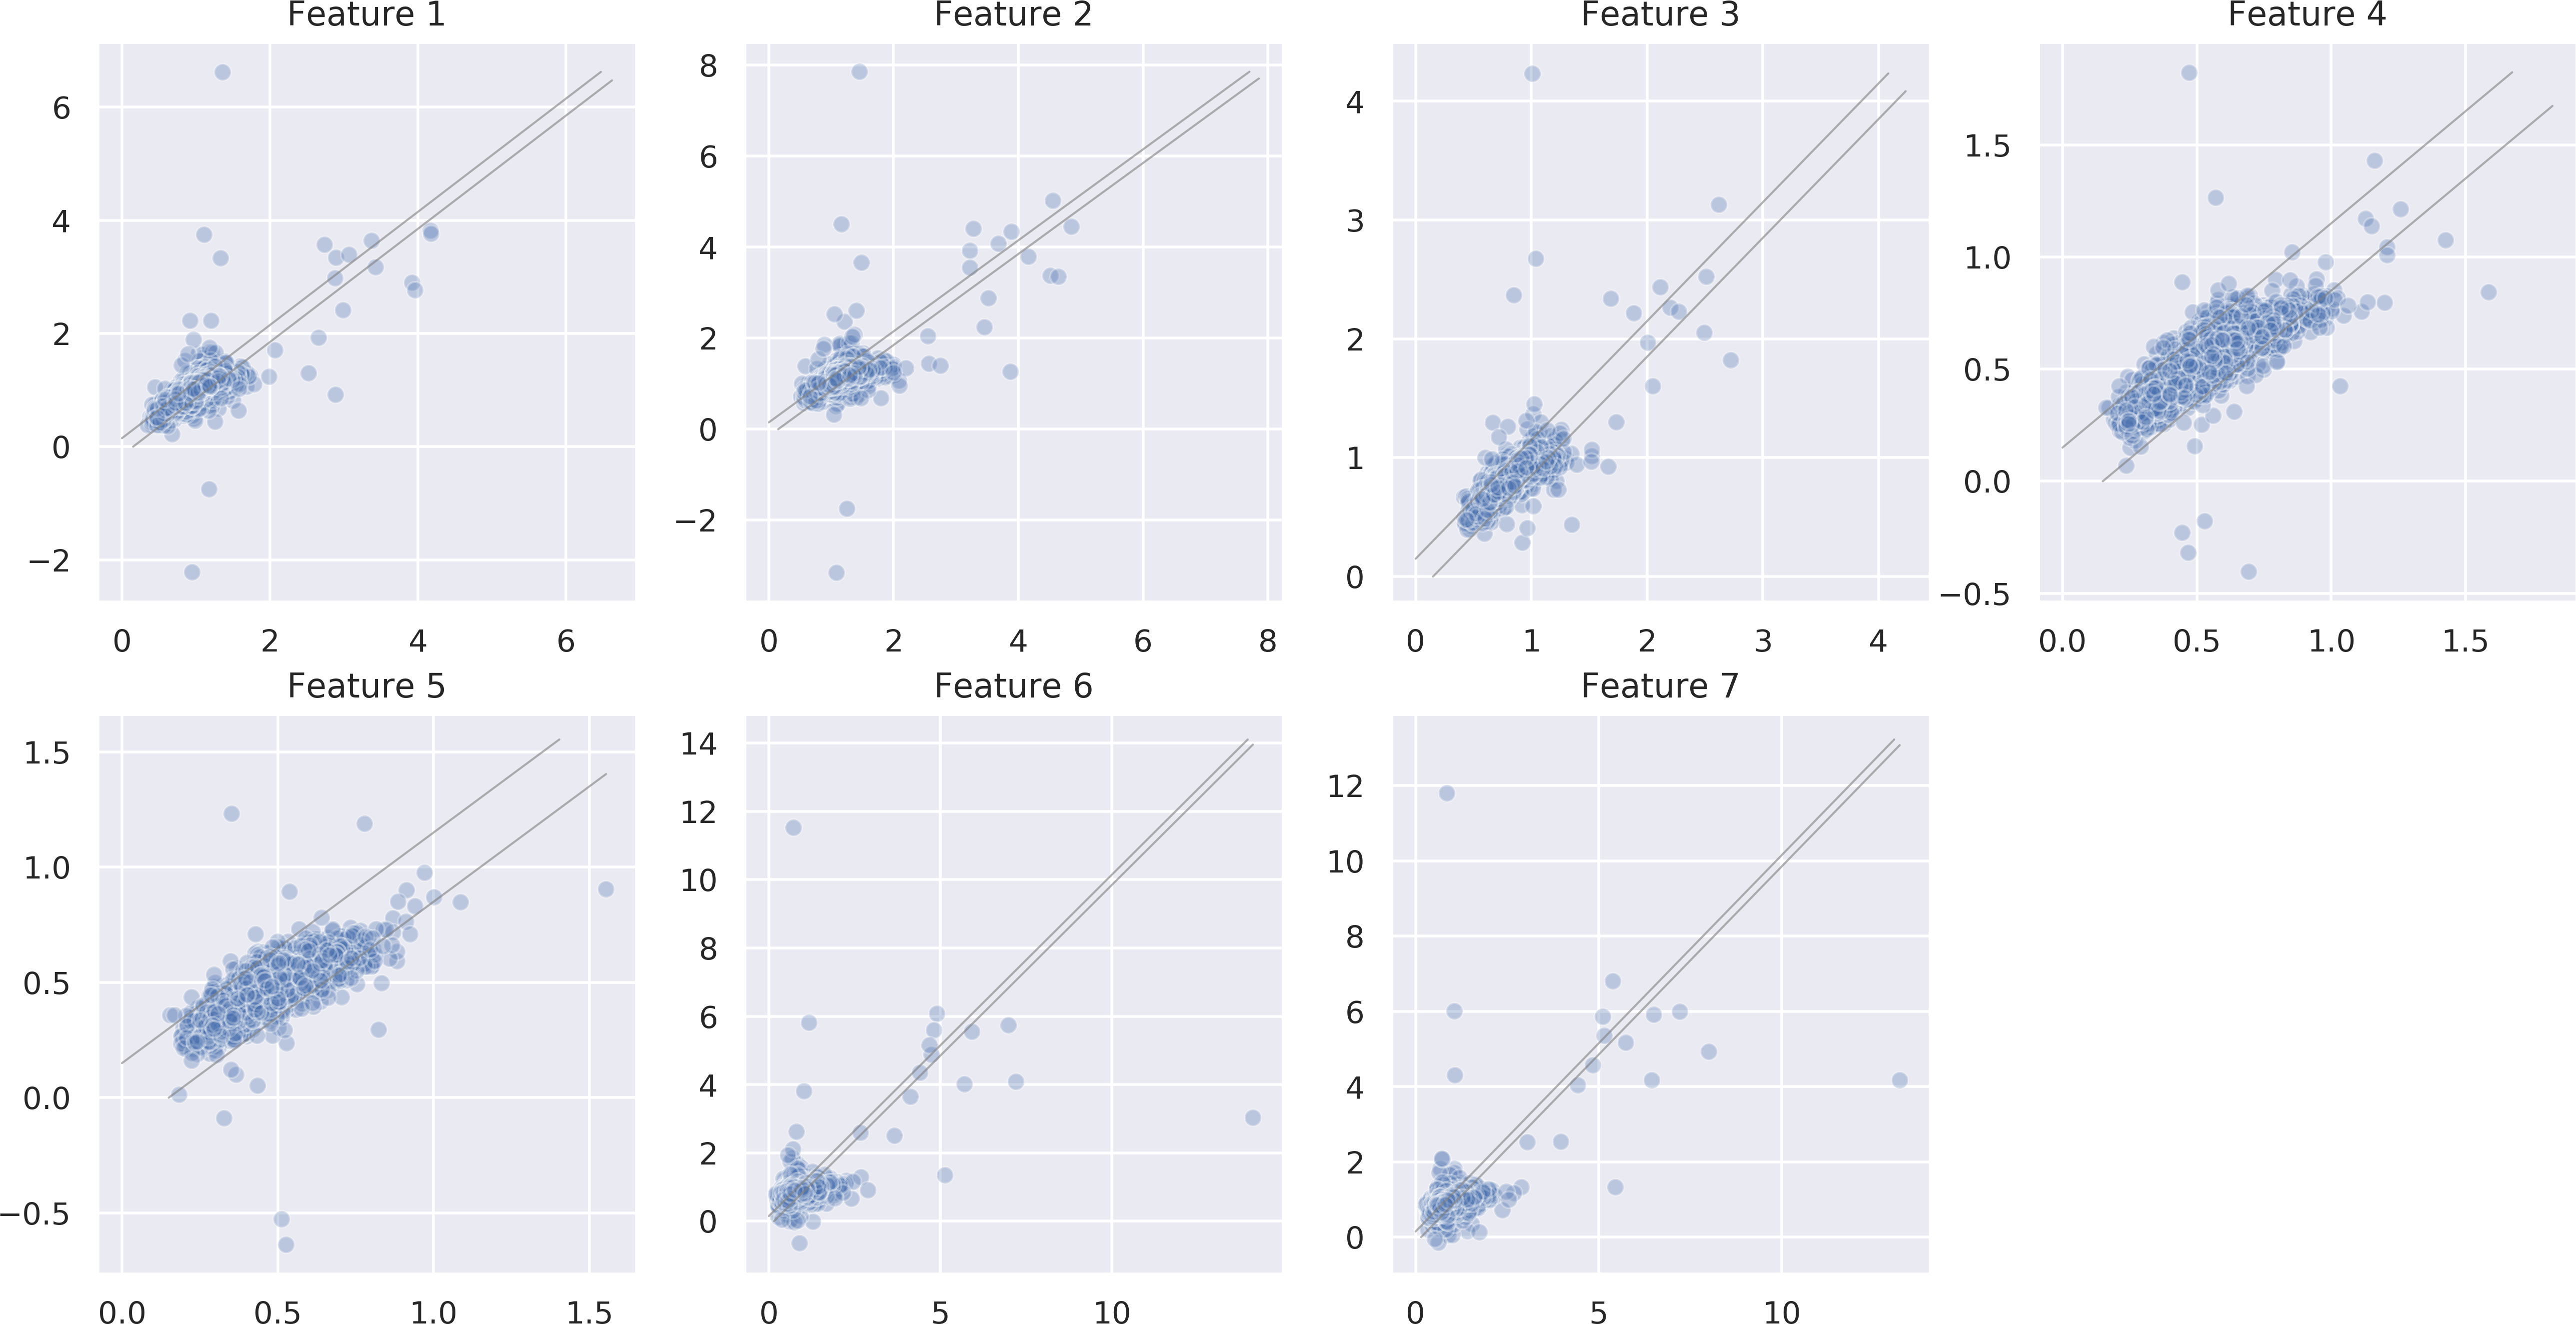
\includegraphics[width=\textwidth]{polyreg_keyval_reg_scatter_complete}
    \caption{\label{fig:polyreg_keyval_reg_scatter_complete} Scatter plots of \(Y_\text{true}\) (\(x\)-axis) versus \(Y_\text{pred}\) (\(y\)-axis) from the complete key value dataset for all seven features, as predicted by the \ac{pr} model. Diagonal lines represent the \(\pm0.15\) tolerance for a hit.}
\end{figure}

Although the model with degree 3 was statistically the best, in Figure \ref{fig:polyreg_keyval_reg_scatter_complete} one can clearly see the first signs of overfitting, with some flights predicted to have consumed negative damage.

A limited ability to predict the trend is visible, but the key value dataset appears not to possess sufficient information for an accurate prediction.

\subsection{PR on Key Values and Features} \label{sec:res:polyreg:kvfs}
This \ac{pr} model was also tested for polynomial degrees from 1 to 5 on the dataset comprising key values and features. Again, \(R^2\) increased with each degree for the training data, but peaked at degree 2 for all three dataset sizes before severe overfitting occurred.

Results are shown in Table \ref{tab:polyreg:kvfs}; predictions \(Y_{\text{pred}}\) are plotted against SA66 values \(Y_{\text{true}}\) in Figure \ref{fig:polyreg_keyvalfeat_reg_scatter_complete}.

\begin{table}
    \renewcommand{\arraystretch}{1.4}
    \begin{center}
        \caption{\label{tab:polyreg:kvfs} Results from the \ac{pr} with polynomial degree 2 on key values including features 1, 4 and 6.}
        \begin{tabular}{ >{\bfseries}c c c c c c c }
            \textbf{Dataset} & \multirow{2}{*}{\textbf{Metric}} & \multicolumn{4}{c}{\textbf{Feature number}} & \multirow{2}{*}{\textbf{Mean}} \\
            size &  & 2 & 3 & 5 & 7 \\
            \midrule
            \multirow{2}{*}{Complete}   & \(R^2\) & 0.964 & 0.835 & 0.845 & 0.930 & 0.893 \\
                                        & HR      & 0.997 & 0.991 & 0.999 & 0.919 & 0.976 \\ \cmidrule{2-7}
            \multirow{2}{*}{Reduced}    & \(R^2\) & 0.931 & 0.827 & 0.845 & 0.850 & 0.863\\
                                        & HR      & 0.995 & 0.992 & 1.000 & 0.901 & 0.972 \\ \cmidrule{2-7}
            \multirow{2}{*}{Minimal}    & \(R^2\) & 0.958 & 0.715 & 0.835 & 0.301 & 0.702 \\
                                        & HR      & 0.993 & 0.980 & 0.993 & 0.901 & 0.967 \\
        \end{tabular}
    \end{center}
\end{table}

\begin{figure}[tb!]
    \centering
    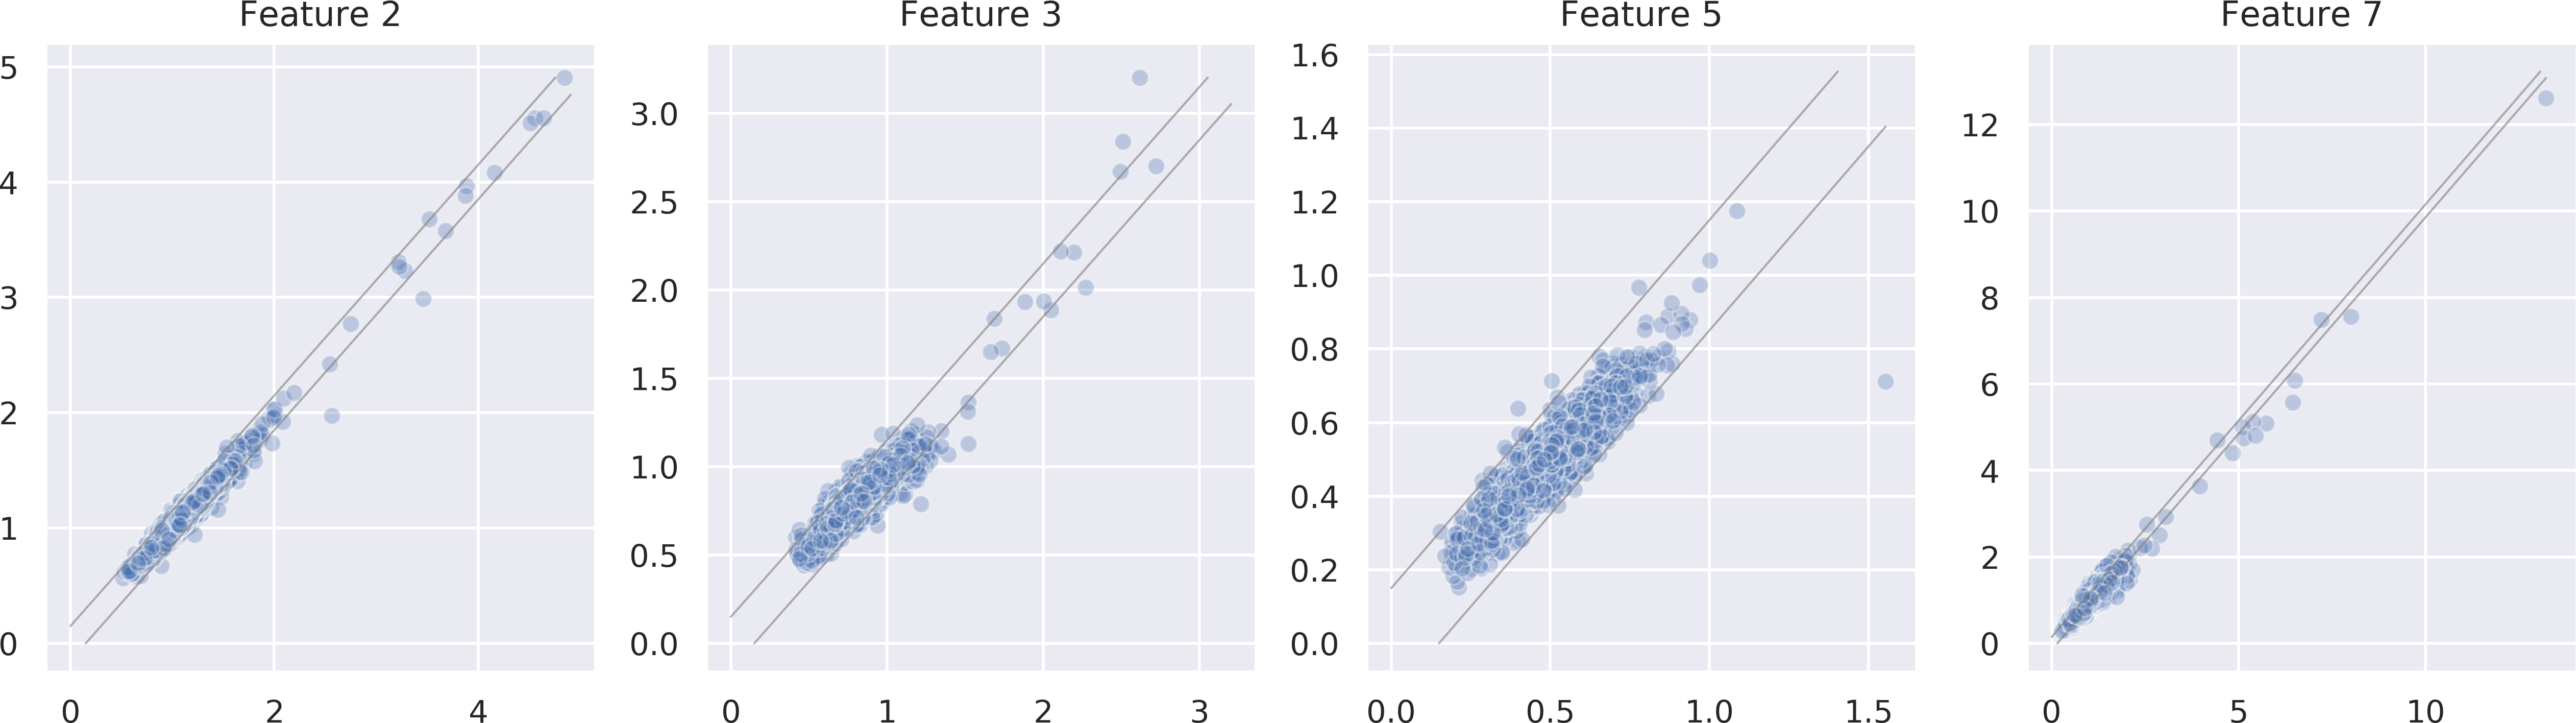
\includegraphics[width=\textwidth]{polyreg_keyvalfeat_reg_scatter_complete}
    \caption{\label{fig:polyreg_keyvalfeat_reg_scatter_complete} Scatter plots of \(Y_\text{true}\) (\(x\)-axis) versus \(Y_\text{pred}\) (\(y\)-axis) from the complete dataset comprising key values and features 1, 4 and 6, showing the \ac{pr} model's damage prediction for features 2, 3, 5 and 7. Diagonal lines represent the \(\pm0.15\) tolerance for a hit.}
\end{figure}

The \ac{pr} model, in combination with the key value dataset including features 1, 4 and 6, displays high MHR and \(R^2\) scores despite its extremely short training time. The scatter plots (Figure \ref{fig:polyreg_keyvalfeat_reg_scatter_complete}) show an obvious tendency towards the line \(x = y\) with almost all data points within the \(\pm0.15\) hit tolerance.

The high \(R^2\) score for all three dataset sizes also indicates good scalability.

% \begin{figure}[tb!]
%     \centering
%     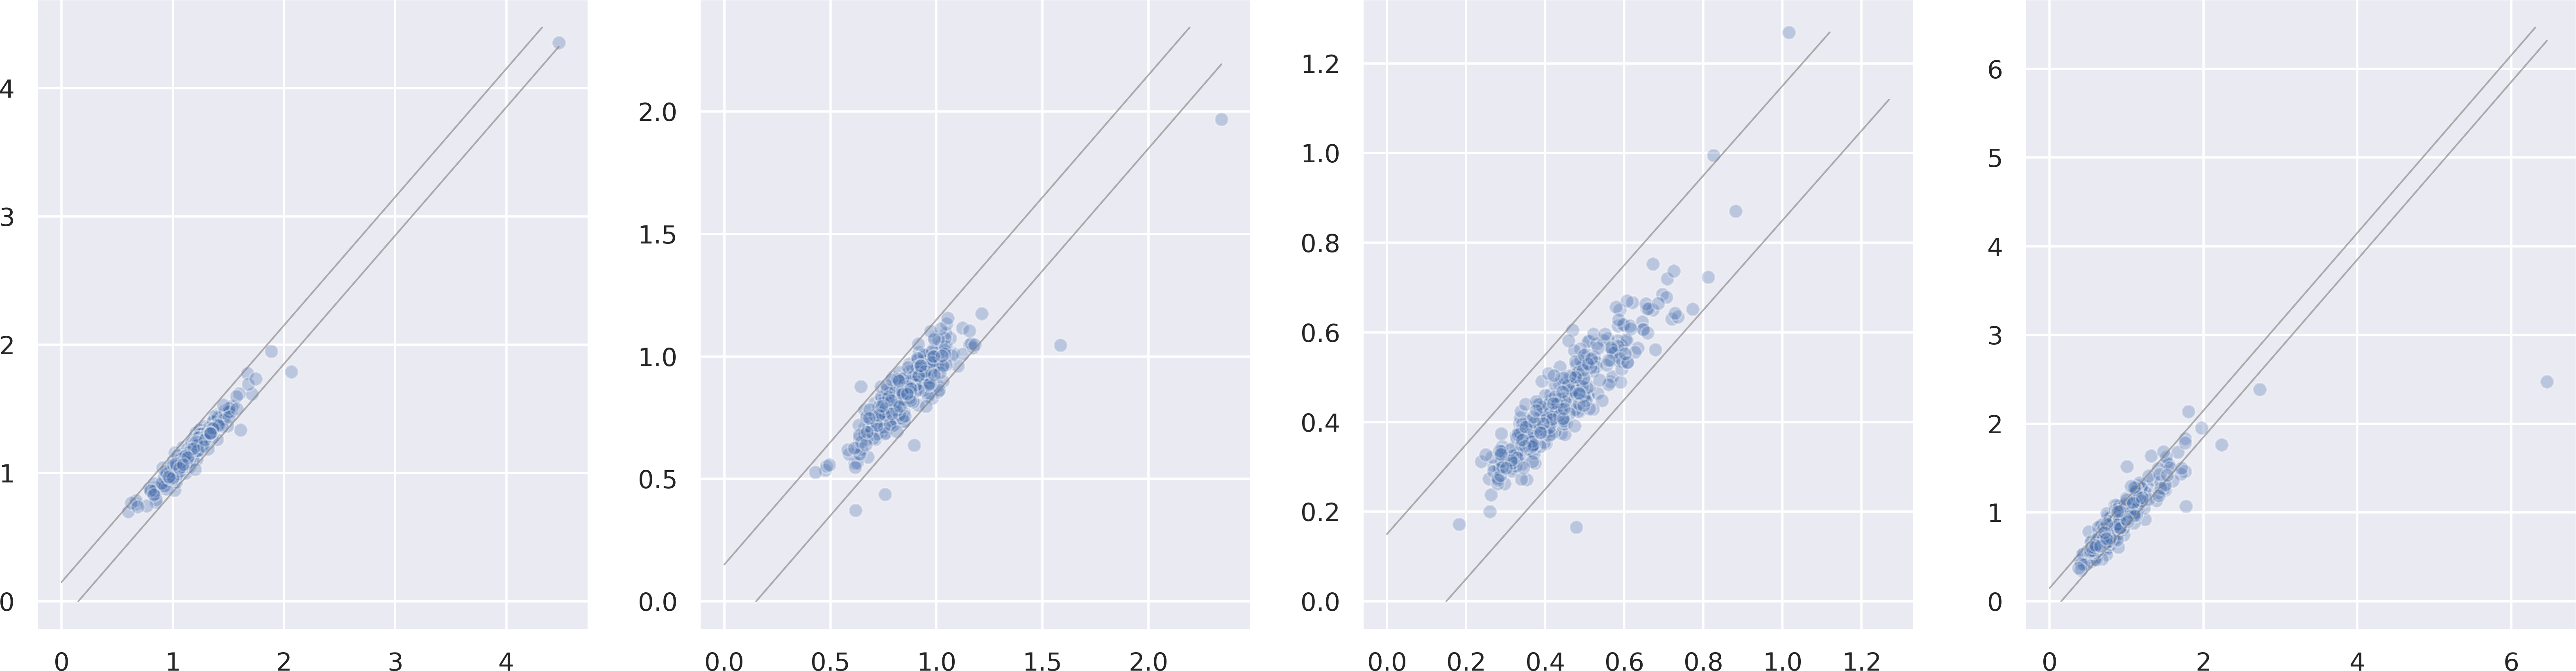
\includegraphics[width=\textwidth]{polyreg_keyvalfeat_reg_scatter_vred}
%     \caption{\label{fig:polyreg_keyvalfeat_reg_scatter_vred} Scatter plots of \(Y_\text{true}\) (\(x\)-axis) versus \(Y_\text{pred}\) (\(y\)-axis) from the minimal dataset comprising key values and features 1, 4 and 6, showing the \ac{pr} model's damage prediction for features 2, 3, 5 and 7. Diagonal lines represent the \(\pm0.15\) tolerance for a hit.}
% \end{figure}

\subsection{MLP Regression on Key Values} \label{sec:res:mlp_kvs}
The \ac{mlp} model was constructed with one to four hidden layers containing 100 perceptrons each; scores peaked for all dataset sizes on the model with two hidden layers.

Results for this model are shown in Table \ref{tab:mlpreg:kvs}; predictions \(Y_{\text{pred}}\) are plotted against SA66 values \(Y_{\text{true}}\) in Figure \ref{fig:mlp_keyval_reg_scatter}.

\begin{table}
    \renewcommand{\arraystretch}{1.4}
    \begin{center}
        \caption{\label{tab:mlpreg:kvs} Results from the \ac{mlp} regression with two hidden layers on the key value dataset.}
        \begin{tabular}{ >{\bfseries}c c c c c c c c c c }
            \textbf{Dataset} & \multirow{2}{*}{\textbf{Metric}} & \multicolumn{7}{c}{\textbf{Feature number}} & \multirow{2}{*}{\textbf{Mean}} \\
            size &  & 1 & 2 & 3 & 4 & 5 & 6 & 7 \\
            \midrule
            \multirow{2}{*}{Complete}   & \(R^2\) & 0.558 & 0.397 & 0.619 & 0.705 & 0.618 & 0.173 & 0.282 & 0.479 \\
                                        & HR      & 0.862 & 0.801 & 0.968 & 0.979 & 0.989 & 0.527 & 0.545 & 0.810 \\ \cmidrule{2-10}
            \multirow{2}{*}{Reduced}    & \(R^2\) & 0.212 & -0.245 & 0.524 & 0.689 & 0.546 & -0.228 & -0.113 & 0.198 \\
                                        & HR      & 0.789 & 0.691 & 0.951 & 0.975 & 0.979 & 0.473 & 0.483 & 0.763 \\ \cmidrule{2-10}
            \multirow{2}{*}{Minimal}    & \(R^2\) & -0.155 & -1.05 & -0.048 & 0.467 & 0.321 & -1.579 & -2.246 & -0.613 \\
                                        & HR      & 0.788 & 0.709 & 0.934 & 0.967 & 0.987 & 0.474 & 0.48 & 0.763 \\
        \end{tabular}
    \end{center}
\end{table}

\begin{figure}[tb!]
    \centering
    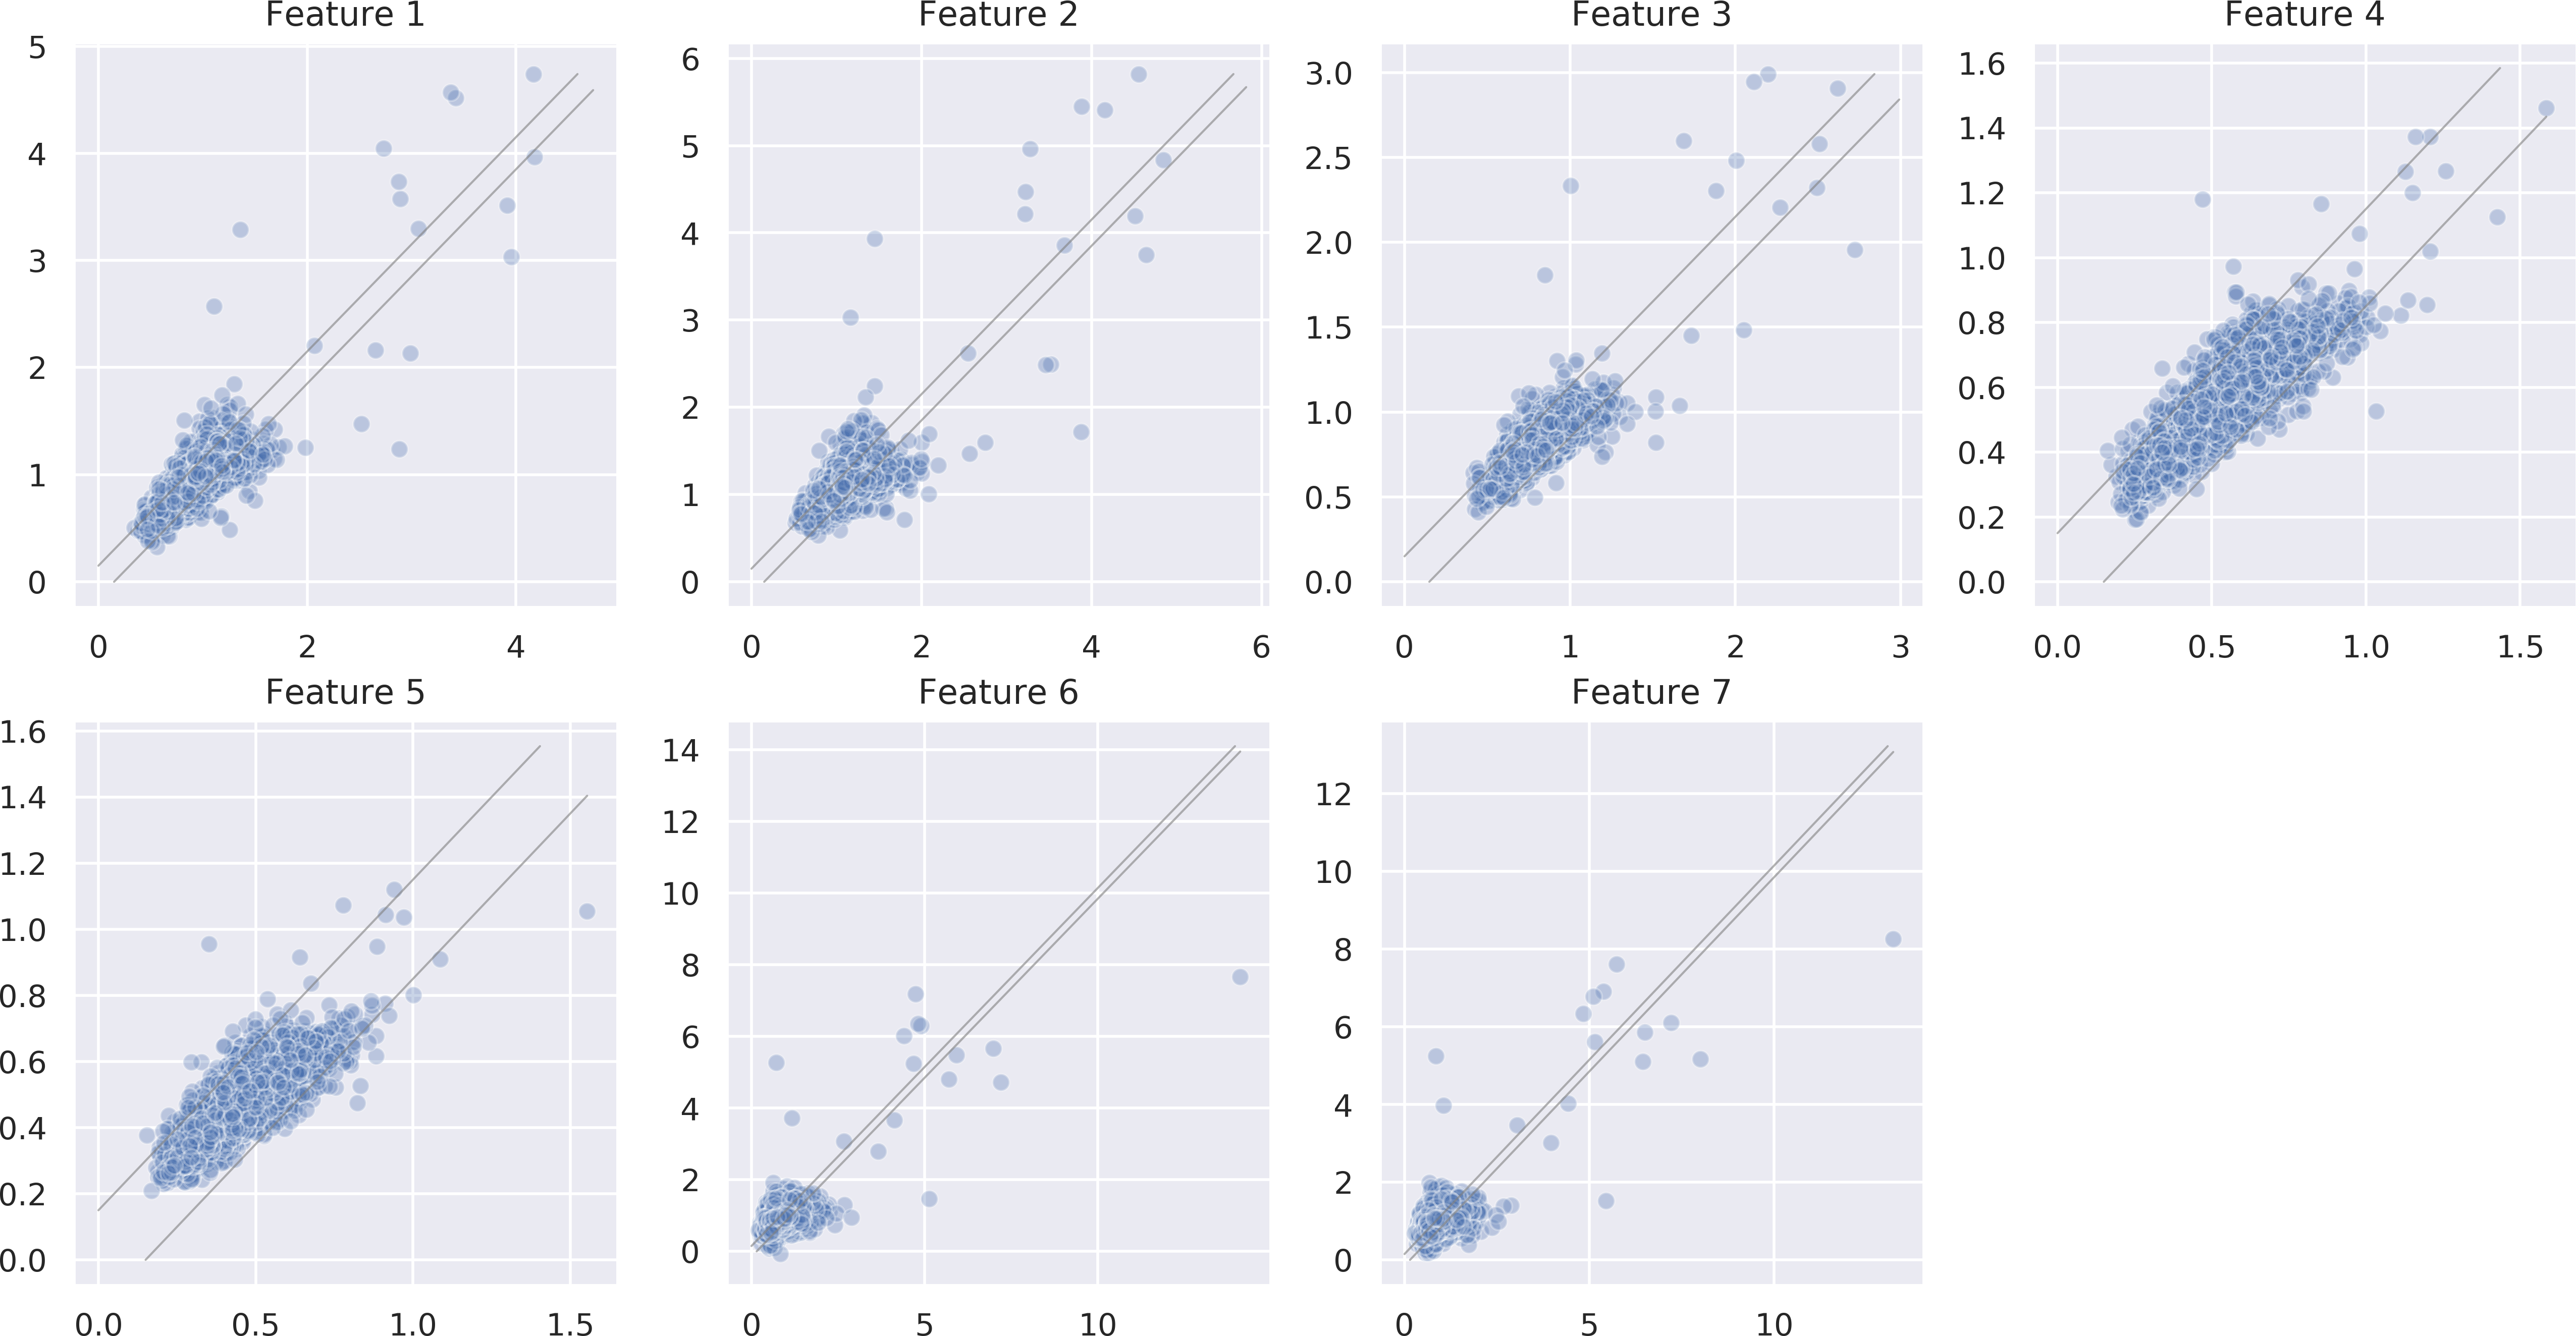
\includegraphics[width=\textwidth]{mlp_keyval_reg_scatter}
    \caption{\label{fig:mlp_keyval_reg_scatter} Scatter plots of \(Y_\text{true}\) (\(x\)-axis) versus \(Y_\text{pred}\) (\(y\)-axis) from the complete key value dataset for all seven features, as predicted by the \ac{mlp}. Diagonal lines represent the \(\pm0.15\) tolerance for a hit.}
\end{figure}

One anomalous flight with over 13 cycles of damage in both features 6 and 7 is predicted with moderate success, as visible in Figure \ref{fig:mlp_keyval_reg_scatter}, as it is correctly predicted to be the most damaging flight. The feature 7 prediction is marginally above the maximum damage from the training dataset, suggesting that the \ac{mlp} regressor is capable of extrapolating --- albeit not by a great amount in this case --- when trained on key values.

Unfortunately, the spread of the predictions increases greatly as the dataset is reduced resulting in an increasingly poor \(R^2\), for which reason using an \ac{mlp} with the input values contained in this dataset is not recommended for further research.

\subsection{MLP Regression on Key Values and Features} \label{sec:res:mlp_kvfs}
This model was also trained with one to four hidden layers; again, scores peaked for all datasets on the model with two hidden layers.

Results for this model are shown in Table \ref{tab:mlpreg:kvfs}; predictions \(Y_{\text{pred}}\) are plotted against SA66 values \(Y_{\text{true}}\) in Figure \ref{fig:mlp_keyvalfeat_reg_scatter}.

\begin{table}
    \renewcommand{\arraystretch}{1.4}
    \begin{center}
        \caption{\label{tab:mlpreg:kvfs} Results from the \ac{mlp} regression on key values including features 1, 4 and 6.}
        \begin{tabular}{ >{\bfseries}c c c c c c c }
            \textbf{Dataset} & \multirow{2}{*}{\textbf{Metric}} & \multicolumn{4}{c}{\textbf{Feature number}} & \multirow{2}{*}{\textbf{Mean}} \\
            size &  & 2 & 3 & 5 & 7 \\
            \midrule
            \multirow{2}{*}{Complete}   & \(R^2\) & 0.956 & 0.803 & 0.850 & 0.920 & 0.882 \\
                                        & HR      & 0.997 & 0.991 & 0.999 & 0.902 & 0.972 \\ \cmidrule{2-7}
            \multirow{2}{*}{Reduced}    & \(R^2\) & 0.963 & 0.792 & 0.818 & 0.868 & 0.861 \\
                                        & HR      & 0.989 & 0.988 & 0.999 & 0.878 & 0.963 \\ \cmidrule{2-7}
            \multirow{2}{*}{Minimal}    & \(R^2\) & 0.901 & 0.719 & 0.708 & 0.849 & 0.794 \\
                                        & HR      & 0.980 & 0.983 & 0.990 & 0.884 & 0.959 \\
        \end{tabular}
    \end{center}
\end{table}

\begin{figure}[tb!]
    \centering
    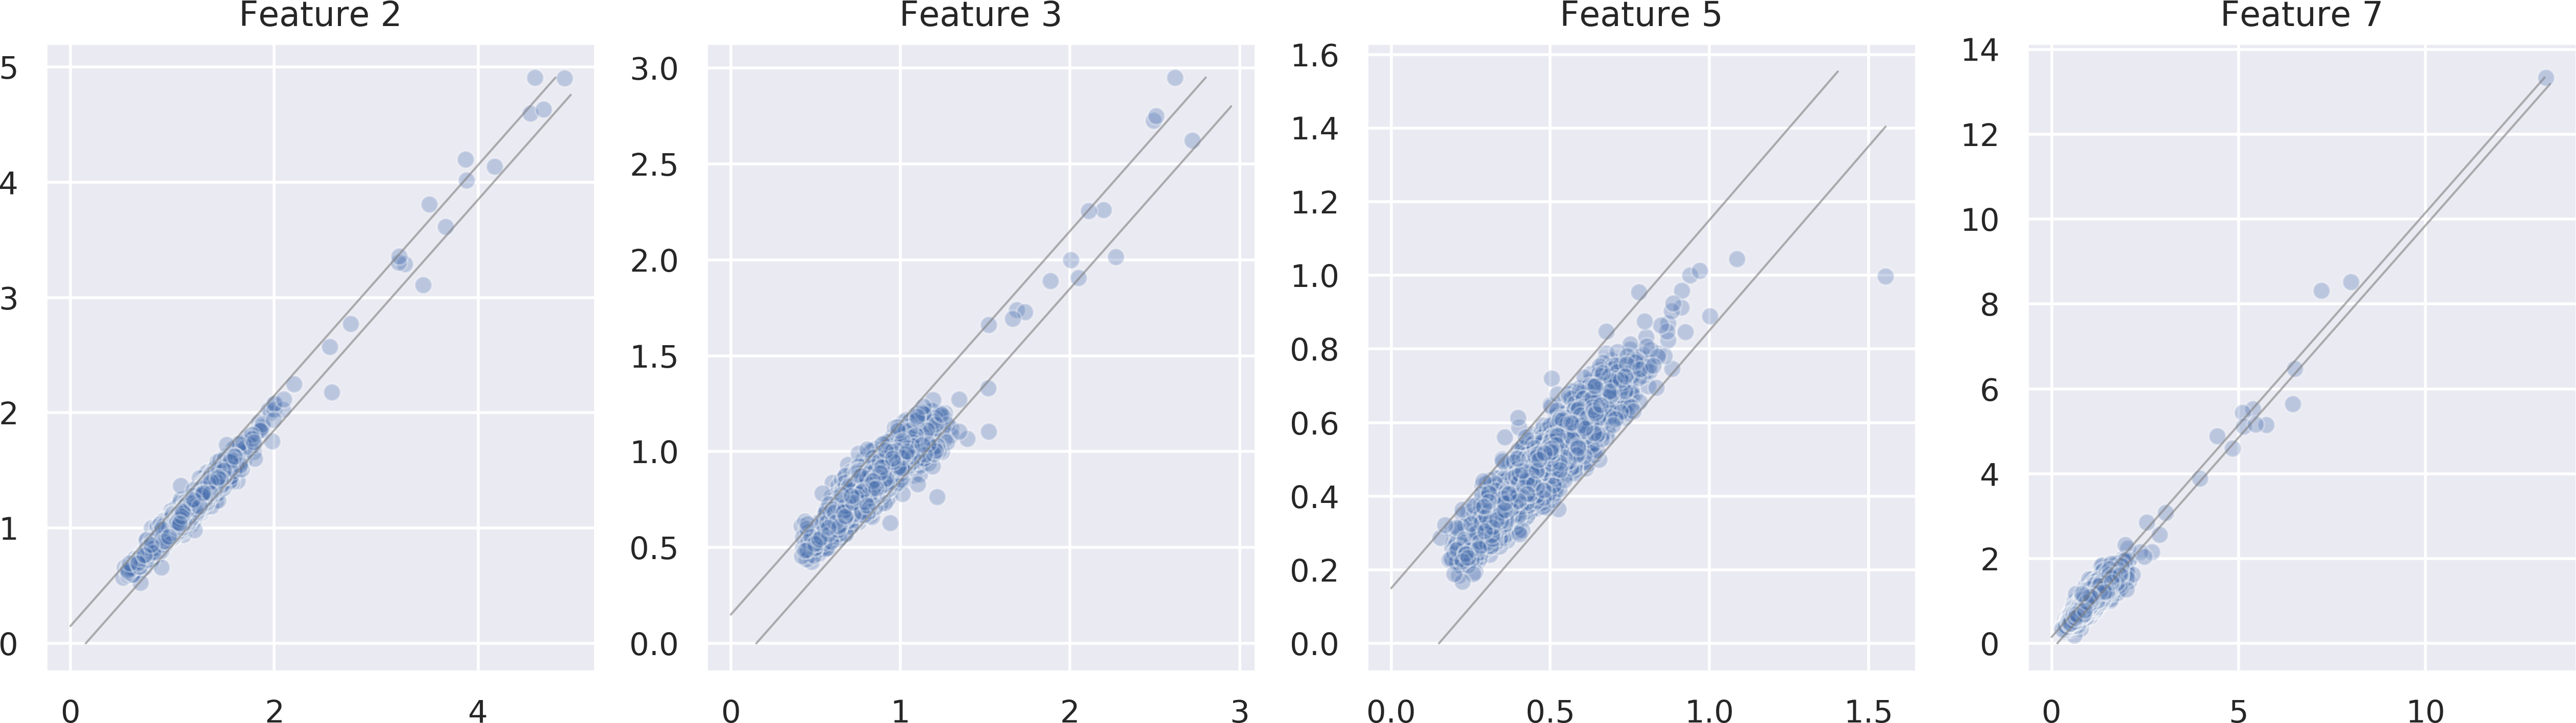
\includegraphics[width=\textwidth]{mlp_keyvalfeat_reg_scatter}
    \caption{\label{fig:mlp_keyvalfeat_reg_scatter} Scatter plots of \(Y_\text{true}\) (\(x\)-axis) versus \(Y_\text{pred}\) (\(y\)-axis) from the complete dataset comprising key values and features 1, 4 and 6, showing features 2, 3, 5 and 7 predicted by the \ac{mlp}. Diagonal lines represent the \(\pm0.15\) tolerance for a hit.}
\end{figure}

This model scores very highly in both MHR and \(R^2\). Visually (Figure \ref{fig:mlp_keyvalfeat_reg_scatter}), the predictions come very close to SA66 values, and the model makes a near-perfect prediction of even the anomalous high-damage flight.

With its short training time, the \ac{mlp} combined with this dataset is highly suitable for further consideration in the research.

\subsection{MLP Regression on Concatenated Multivariate Time Series} \label{sec:res:mlpreg:mts}
This model was also trained with one to four hidden layers; this time, scores peaked for the \ac{mlp} with one hidden layer.

Results for this model are shown in Table \ref{tab:mlpreg:mts}; predictions \(Y_{\text{pred}}\) are plotted against SA66 values \(Y_{\text{true}}\) in Figure \ref{fig:mlp_mts_reg_scatter}.

\begin{table}
    \renewcommand{\arraystretch}{1.4}
    \begin{center}
        \caption{\label{tab:mlpreg:mts} Results from the \ac{mlp} regression on the concatenated multivariate time series.}
        \begin{tabular}{ >{\bfseries}c c c c c c c c c c }
            \textbf{Dataset} & \multirow{2}{*}{\textbf{Metric}} & \multicolumn{7}{c}{\textbf{Feature number}} & \multirow{2}{*}{\textbf{Mean}} \\
            size &  & 1 & 2 & 3 & 4 & 5 & 6 & 7 \\
            \midrule
            \multirow{2}{*}{Complete}   & \(R^2\) & 0.696 & 0.583 & 0.691 & 0.199 & 0.059 & 0.199 & 0.260 & 0.384 \\
                                        & HR      & 0.892 & 0.816 & 0.977 & 0.903 & 0.959 & 0.516 & 0.512 & 0.796 \\ \cmidrule{2-10}
            \multirow{2}{*}{Reduced}    & \(R^2\) & 0.691 & 0.567 & 0.669 & 0.210 & 0.058 & 0.181 & 0.237 & 0.373 \\
                                        & HR      & 0.892 & 0.817 & 0.972 & 0.904 & 0.959 & 0.525 & 0.521 & 0.799 \\ \cmidrule{2-10}
            \multirow{2}{*}{Minimal}    & \(R^2\) & 0.664 & 0.559 & 0.666 & 0.126 & 0.013 & 0.163 & 0.228 & 0.346 \\
                                        & HR      & 0.876 & 0.794 & 0.973 & 0.897 & 0.956 & 0.507 & 0.516 & 0.788 \\
        \end{tabular}
    \end{center}
\end{table}

\begin{figure}[tb!]
    \centering
    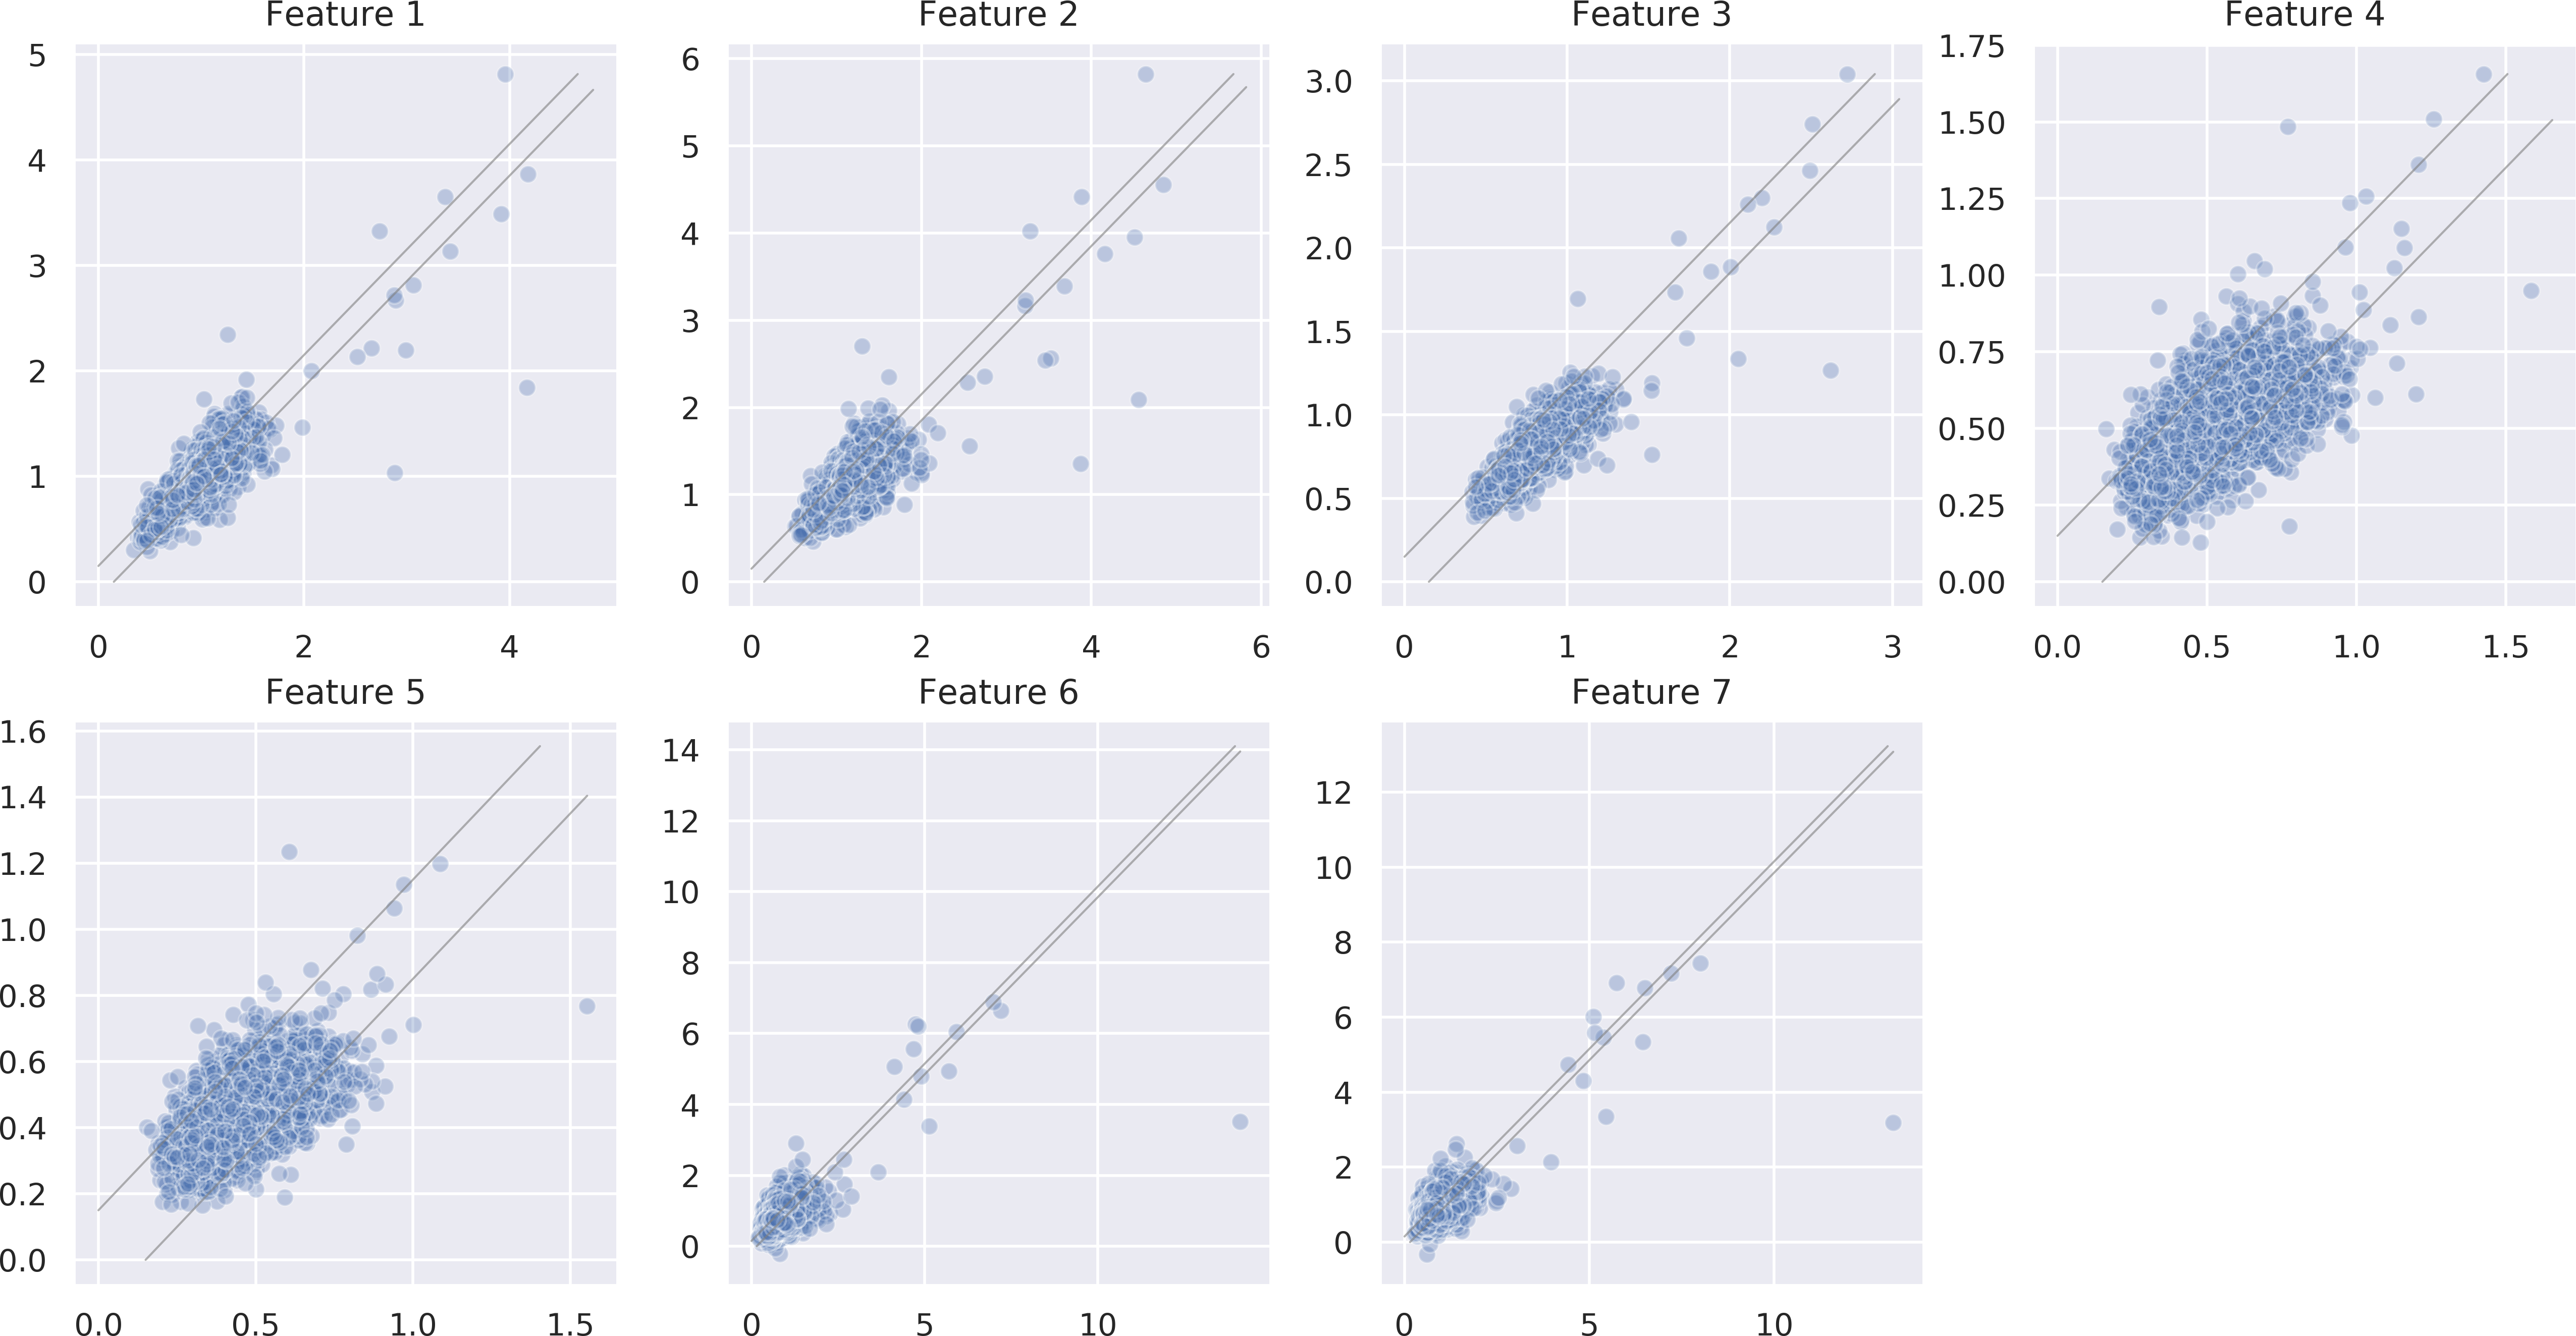
\includegraphics[width=\textwidth]{mlp_mts_reg_scatter}
    \caption{\label{fig:mlp_mts_reg_scatter} Scatter plots of \(Y_\text{true}\) (\(x\)-axis) versus \(Y_\text{pred}\) (\(y\)-axis) from the complete concatenated time series dataset for all seven features, as predicted by the \ac{mlp}. Diagonal lines represent the \(\pm0.15\) tolerance for a hit.}
\end{figure}

The \ac{mlp}'s performance on the concatenated time series dataset is comparable to its performance on the key value dataset in terms of MHR. The scatter plot (Figure \ref{fig:mlp_mts_reg_scatter}) shows a worse fit in terms of spread on features 4 and 5 in comparison to the key value model.

The results and plots from this \ac{mlp} model show that it is clearly capable of accurately predicting the trend in the data. The model performs well on all three datasets in all three sizes.

\subsection{CNN Regression on Multivariate Time Series} \label{sec:res:cnn:reg}
Results from this model are shown in Table \ref{tab:inc:lin}; predictions \(Y_{\text{pred}}\) are plotted against SA66 values \(Y_{\text{true}}\) in Figure \ref{fig:incep_mts_reg_scatter}.

\begin{table}
    \renewcommand{\arraystretch}{1.4}
    \begin{center}
        \caption{\label{tab:inc:lin} Results from the \ac{cnn} regression on multivariate time series.}
        \begin{tabular}{ >{\bfseries}c c c c c c c c c c }
            \textbf{Dataset} & \multirow{2}{*}{\textbf{Metric}} & \multicolumn{7}{c}{\textbf{Feature number}} & \multirow{2}{*}{\textbf{Mean}} \\
            size &  & 1 & 2 & 3 & 4 & 5 & 6 & 7 \\
            \midrule
            \multirow{2}{*}{Complete}   & \(R^2\) & 0.732 & 0.653 & 0.702 & 0.310 & 0.306 & 0.365 & 0.392 & 0.494 \\
                                        & HR      & 0.870 & 0.799 & 0.959 & 0.826 & 0.919 & 0.445 & 0.432 & 0.750 \\ \cmidrule{2-10}
            \multirow{2}{*}{Reduced}    & \(R^2\) & 0.502 & 0.344 & 0.594 & 0.221 & 0.204 & 0.258 & 0.327 & 0.350 \\
                                        & HR      & 0.803 & 0.718 & 0.903 & 0.792 & 0.889 & 0.475 & 0.459 & 0.720 \\ \cmidrule{2-10}
            \multirow{2}{*}{Minimal}    & \(R^2\) & 0.610 & 0.516 & 0.277 & -0.503 & -1.142 & 0.160 & 0.164 & 0.012 \\
                                        & HR      & 0.715 & 0.649 & 0.702 & 0.480 & 0.497 & 0.344 & 0.361 & 0.535 \\
        \end{tabular}
    \end{center}
\end{table}

\begin{figure}[tb!]
    \centering
    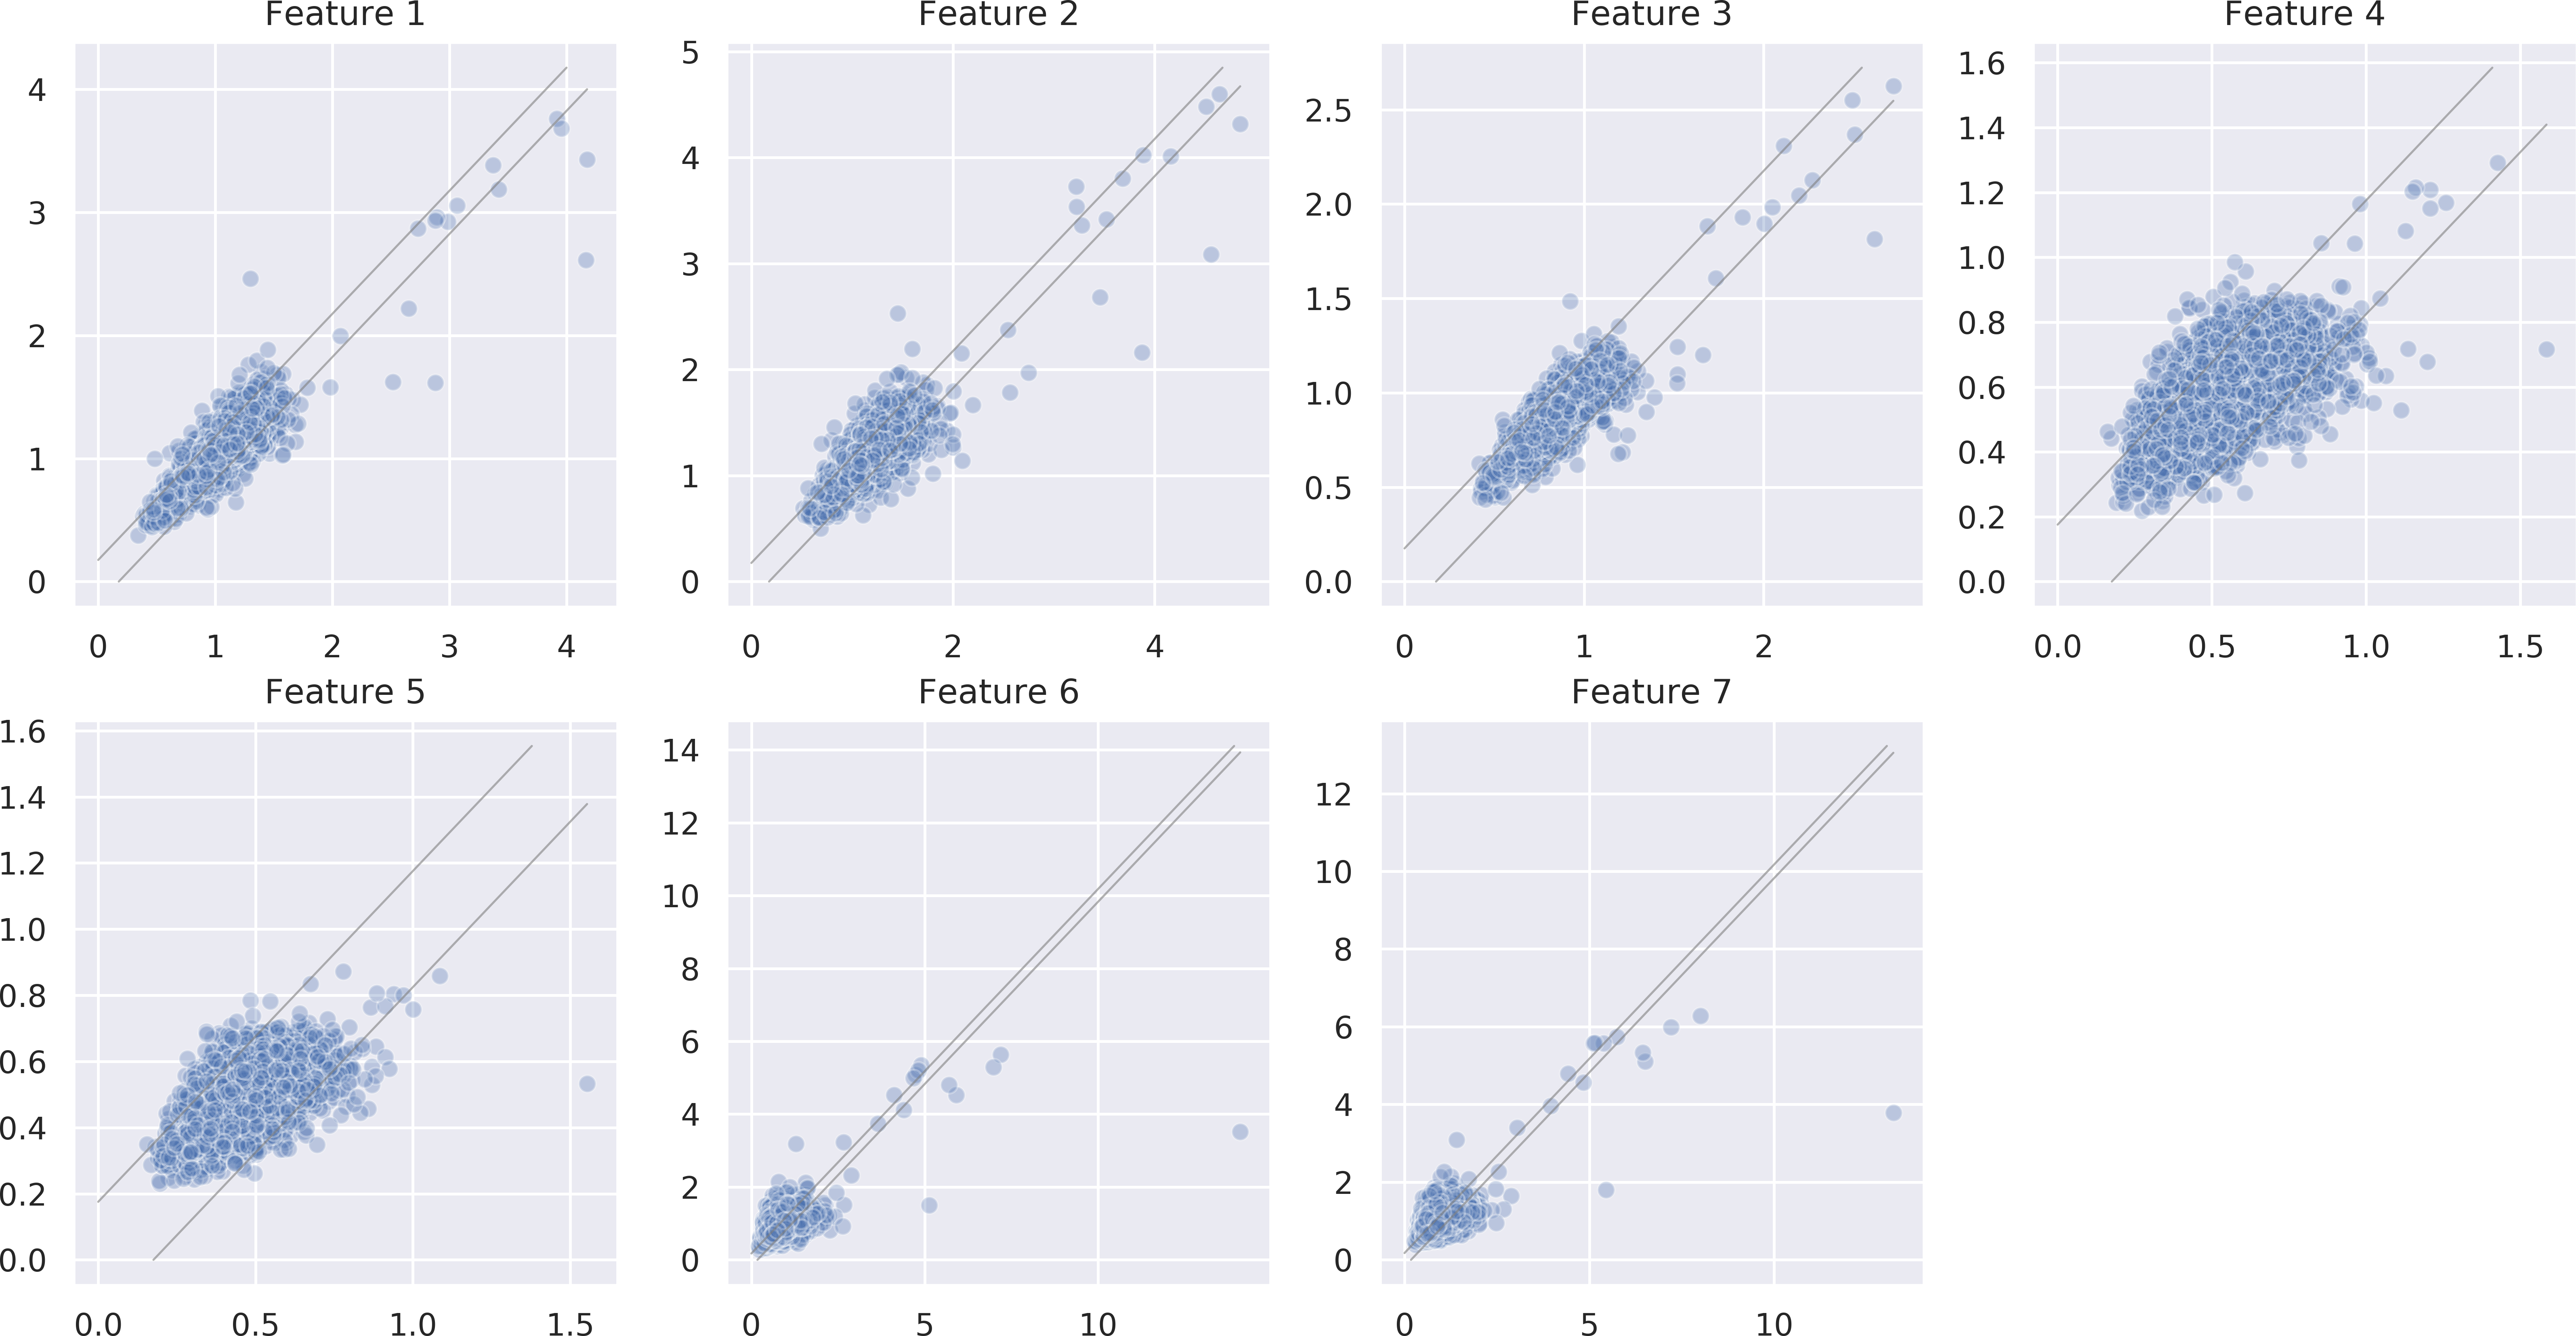
\includegraphics[width=\textwidth]{incep_mts_reg_scatter}
    \caption{\label{fig:incep_mts_reg_scatter} Scatter plots of \(Y_\text{true}\) (\(x\)-axis) versus \(Y_\text{pred}\) (\(y\)-axis) from the complete \ac{mts} dataset for all seven features, as predicted by the \ac{cnn} regressor. Diagonal lines represent the \(\pm0.15\) tolerance for a hit.}
\end{figure}

Results from the \ac{cnn} time series regression are promising. Figure \ref{fig:incep_mts_reg_scatter} shows that the model is moderately capable of recognising and predicting a trend in damage from flight data. This ability is most visible in the plots of features 1 to 3. Features 6 and 7, on the other hand, illustrate the model's inability to extrapolate beyond the training data: the anomalous high-damage flight in these features was predicted to consume fewer than 4 cycles. No flights in the training data breached 8 cycles, so the model was not equipped to predict damage beyond this value.

\subsection{CNN Classification on Multivariate Time Series} \label{sec:res:cnn:cls}
Results are shown for the classification task in Table \ref{tab:inc:4cat}; the accuracy of the class predictions in comparison to the SA66 values, calculated as \(\left|Y_\text{pred} - Y_\text{true}\right|\), are shown in Figure \ref{fig:classif_pred_hist}.

\begin{table}
    \renewcommand{\arraystretch}{1.4}
    \begin{center}
        \caption{\label{tab:inc:4cat} Results from the \ac{cnn} classification on multivariate time series.}
        \begin{tabular}{ >{\bfseries}c c c c c c c c c c }
            \textbf{Dataset} & \multirow{2}{*}{\textbf{Metric}} & \multicolumn{7}{c}{\textbf{Feature number}} & \multirow{2}{*}{\textbf{Mean}} \\
            size &  & 1 & 2 & 3 & 4 & 5 & 6 & 7 \\
            \midrule
            \multirow{2}{*}{Complete}   & MAE & 0.439 & 0.507 & 0.500 & 0.596 & 0.651 & 0.742 & 0.755 & 0.599 \\
                                        & HR  & 0.588 & 0.541 & 0.546 & 0.452 & 0.418 & 0.363 & 0.360 & 0.467 \\\cmidrule{2-10}
            \multirow{2}{*}{Reduced}    & MAE & 0.502 & 0.621 & 0.464 & 0.682 & 0.669 & 0.785 & 0.811 & 0.648 \\
                                        & HR  & 0.554 & 0.464 & 0.581 & 0.409 & 0.405 & 0.329 & 0.316 & 0.437 \\ \cmidrule{2-10}
            \multirow{2}{*}{Minimal}    & MAE & 0.560 & 0.695 & 0.623 & 0.801 & 0.798 & 0.927 & 0.894 & 0.757 \\
                                        & HR  & 0.500 & 0.407 & 0.460 & 0.325 & 0.358 & 0.278 & 0.301 & 0.376\\
        \end{tabular}
    \end{center}
\end{table}

\begin{figure}[tb!]
    \centering
    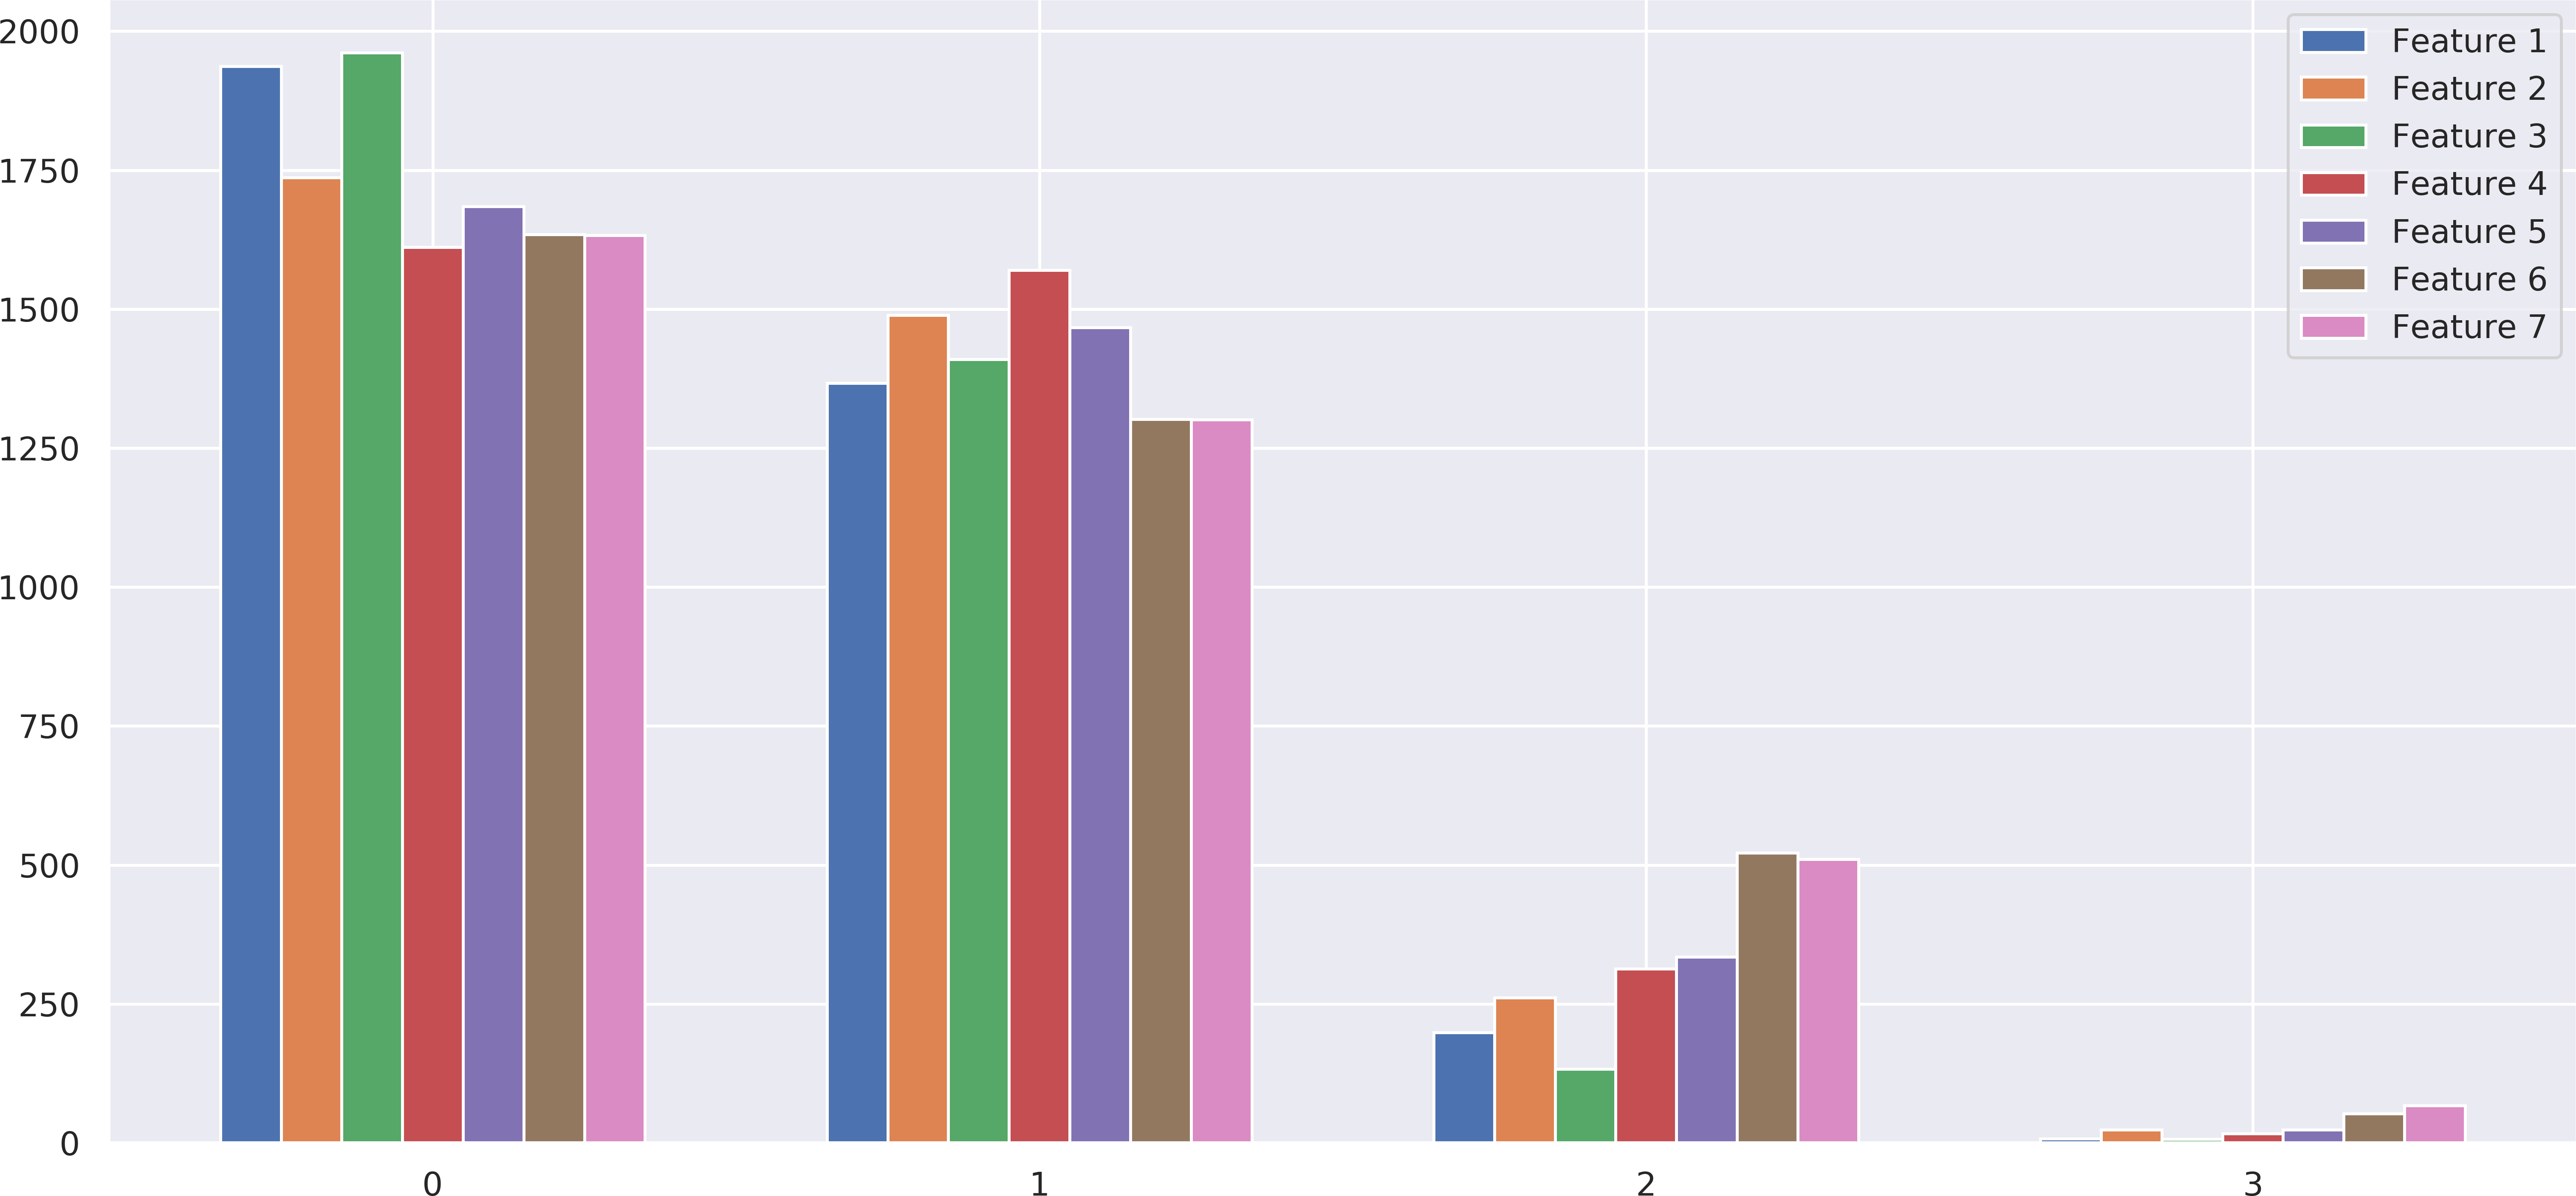
\includegraphics[width=\textwidth]{4cat_err_bar_complete}
    \caption{\label{fig:classif_pred_hist} Bar plot of absolute errors (\(x\)-axis) by feature (colour) from the \ac{cnn} classification model trained with the complete dataset.}
\end{figure}

Results from the classification problem show that the model is capable of correctly labelling a flight as one of four damage classes in fewer than half of cases. Figure \ref{fig:classif_pred_hist} is slightly more optimistic and shows the feature-wise absolute error: most flights are either correct or wrong by one class. While this is promising, in terms of correctly classified flights, the model does not perform substantially better than simply guessing. Furthermore, the bar was set somewhat low by splitting the data into only four classes.

Classification, while an interesting approach, should not be pursued further for damage prediction.

\section{Discussion}
A summary of the main results from all models is shown in Table \ref{tab:model_summary}; the results for all regression models are visualised for comparison in Figure \ref{fig:results_comparison}. Due to its clear inadequacy for the task, the classification model was excluded from this comparison.

\begin{table}
    \renewcommand{\arraystretch}{1.25}
    \begin{center}
        \caption{\label{tab:model_summary} A comparison of mean scores for all seven models and all dataset sizes. Scores reported are the mean across all features for each category. The highest values of measures \(R^2\) and MHR for each dataset size are formatted in bold.}
        \begin{tabular}{ >{\bfseries}m{0.2\textwidth} m{0.15\textwidth} >{\centering}m{0.1\textwidth} >{\centering}m{0.13\textwidth} >{\centering}m{0.13\textwidth} >{\centering\arraybackslash}m{0.13\textwidth} }
            \multirow{2}{*}{\textbf{Model}} & \multirow{2}{*}{\textbf{Dataset}} & \multirow{2}{*}{\textbf{Metric}} & \multicolumn{3}{c}{\textbf{Dataset Size}} \\
            & & & complete & reduced & minimal \\
            \midrule
            \multirow{4}{=}{Polynomial regression}  & \multirow{2}{=}{Key values}               & \(R^2\)   &
            0.254 & 0.136 & -0.069 \\
                                                    &                                           & MHR       &
            0.810 & 0.791 & 0.741 \\ \cmidrule{2-6}
                                                    & \multirow{2}{=}{Key values and features}  & \(R^2\)   &
            \textbf{0.893} & \textbf{0.863} & 0.702 \\
                                                    &                                           & MHR       &
            \textbf{0.976} & \textbf{0.972} & \textbf{0.967} \\ \cmidrule{1-6}
            \multirow{6}{=}{MLP regression}         & \multirow{2}{=}{Key values}               & \(R^2\)   &
            0.479 & 0.198 & -0.612 \\
                                                    &                                           & MHR       &
            0.810 & 0.763 & 0.763 \\ \cmidrule{2-6}
                                                    & \multirow{2}{=}{Key values and features}  & \(R^2\)   &
            0.882 & 0.861 & \textbf{0.794} \\
                                                    &                                           & MHR       &
            0.972 & 0.963 & 0.959 \\ \cmidrule{2-6}
                                                    & \multirow{2}{=}{Concatenated time series} & \(R^2\)   &
            0.384 & 0.373 & 0.346 \\
                                                    &                                           & MHR       &
            0.796 & 0.799 & 0.788 \\ \cmidrule{1-6}
            \multirow{2}{=}{CNN regression}         & \multirow{2}{=}{Multivariate time series} & \(R^2\)   &
            0.494 & 0.350 & 0.012 \\
                                                    &                                           & MHR       &
            0.750 & 0.720 & 0.535 \\ \cmidrule{1-6}
                \multirow{2}{=}{CNN classification} & \multirow{2}{=}{Multivariate time series} & MAE   &
            0.599 & 0.648 & 0.757 \\
                                                    &                                           & MHR       &
            0.467 & 0.437 & 0.376 \\
        \end{tabular}
    \end{center}
\end{table}

\begin{figure}[tb!]
    \centering
    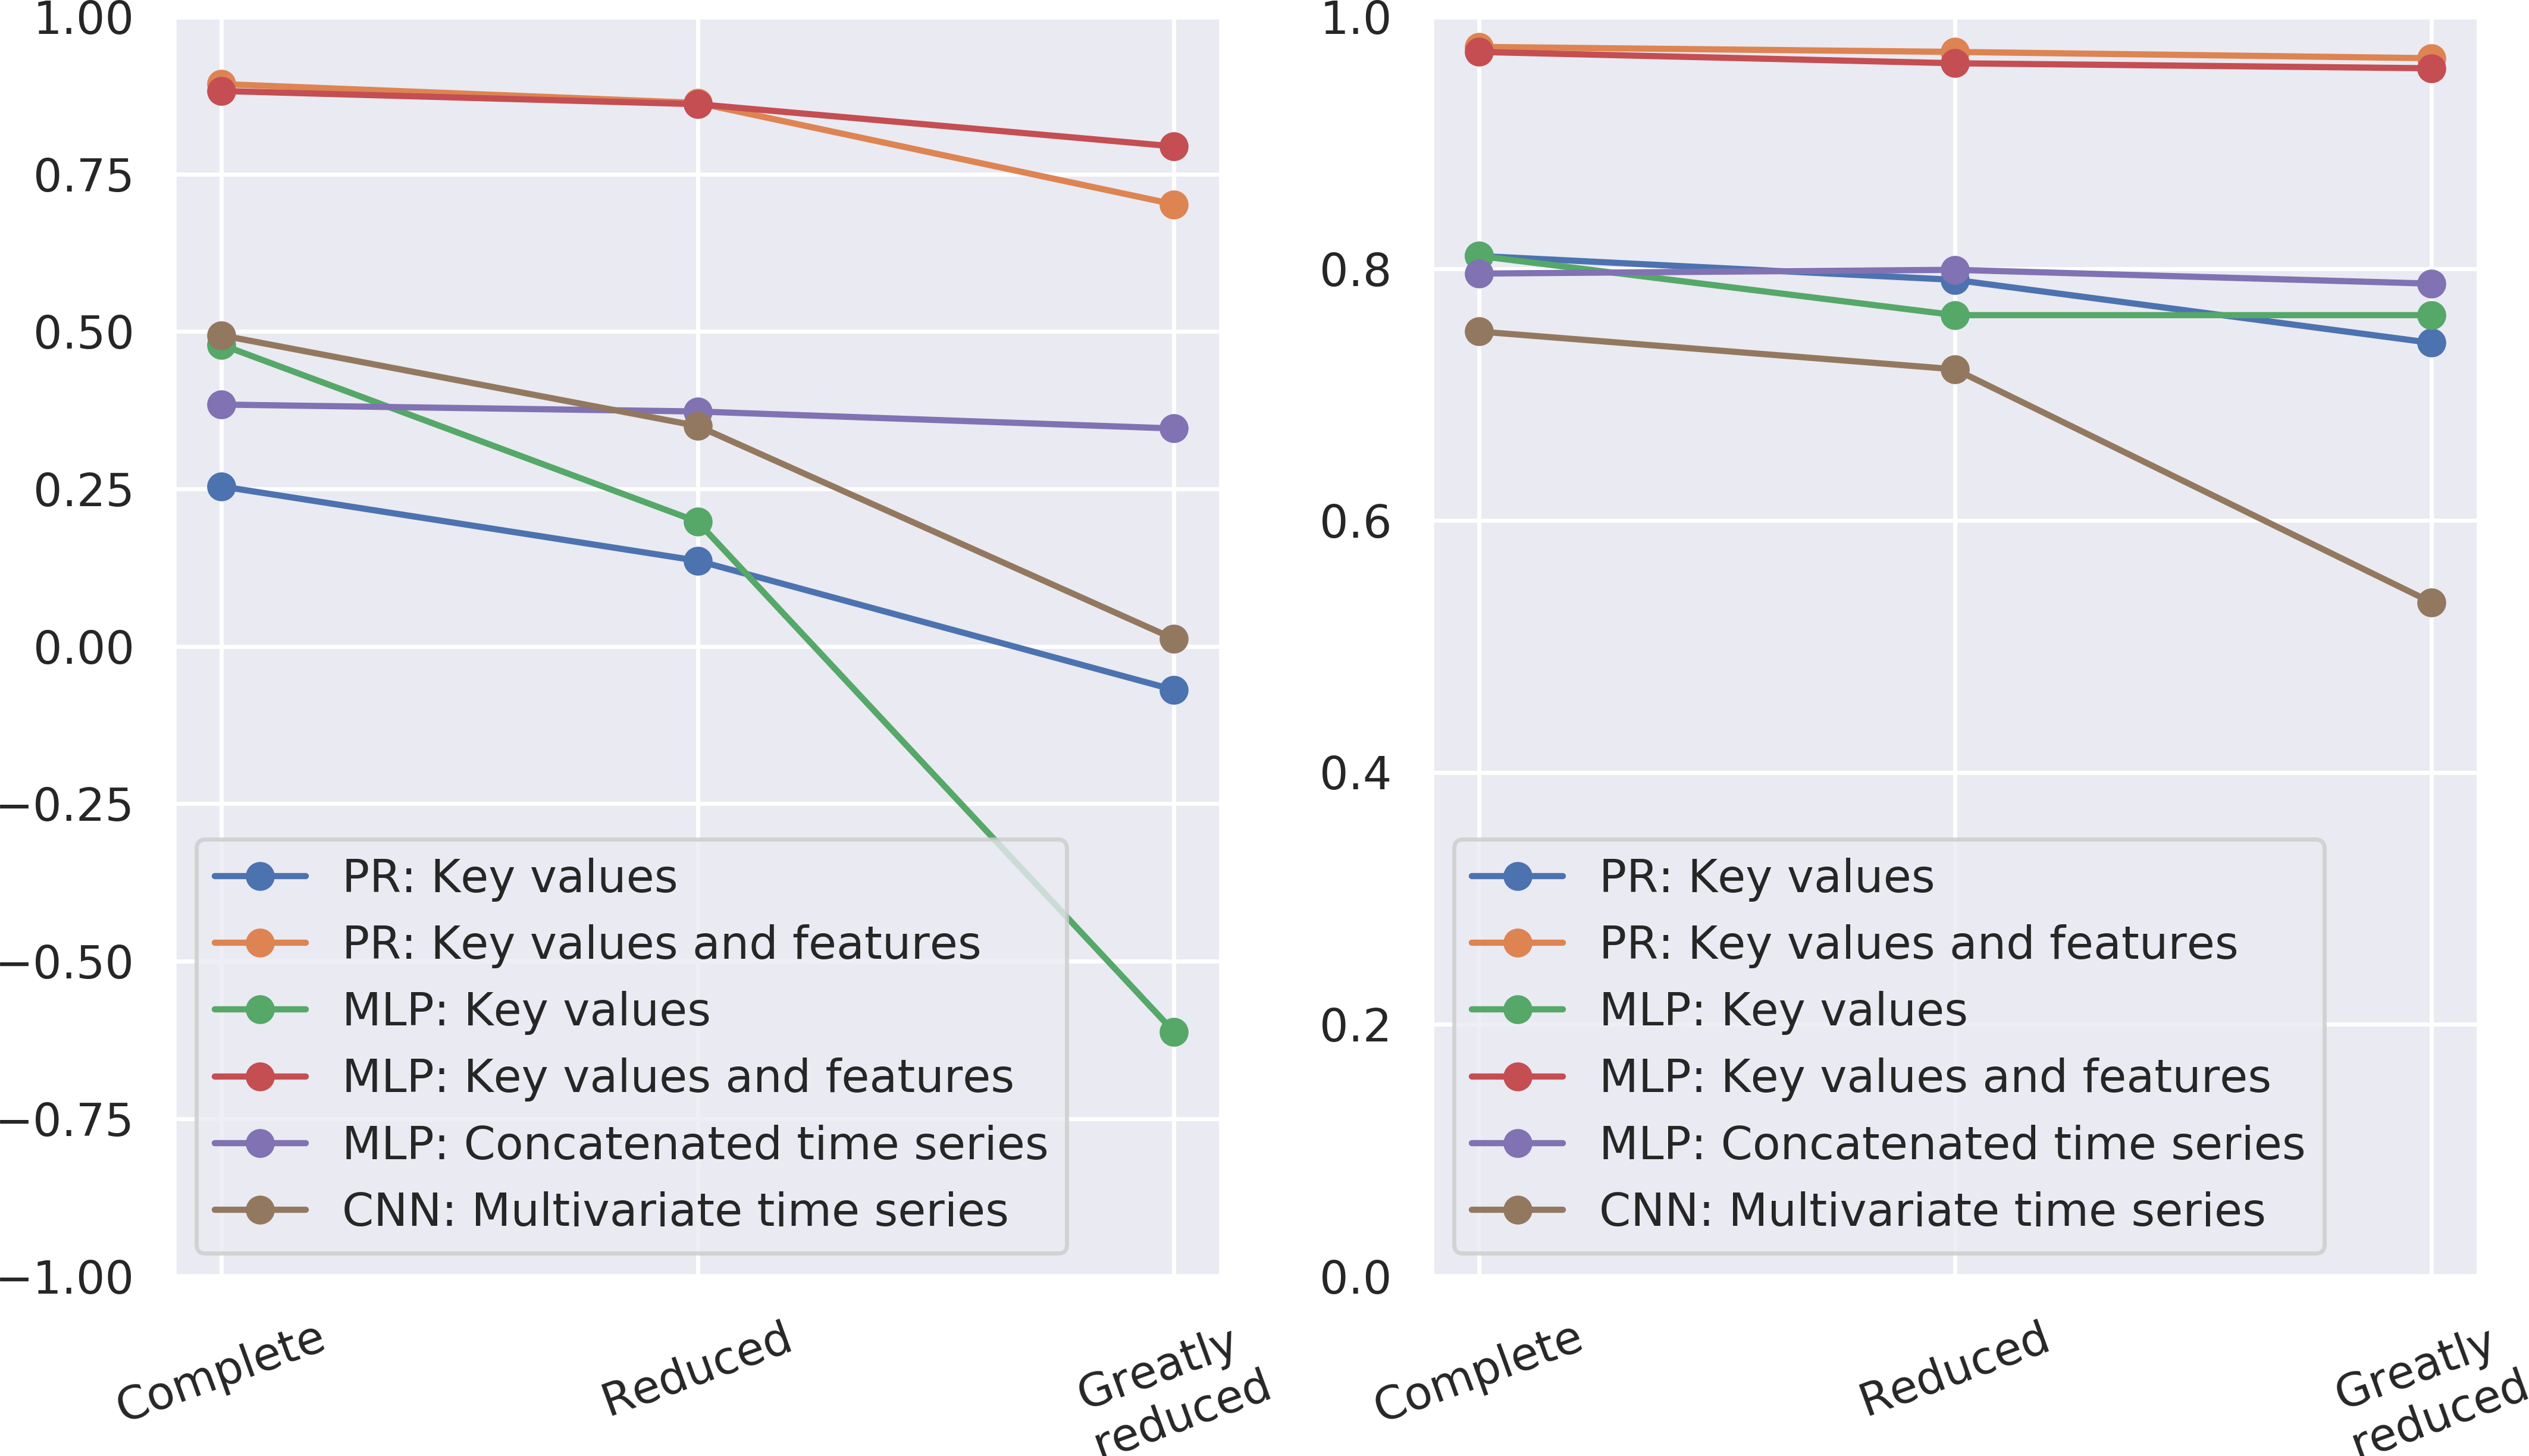
\includegraphics[width=\textwidth]{final_results}
    \caption{\label{fig:results_comparison} A comparison of the final results for all regression models. Left: \(R^2\) score for each model versus dataset size. Right: The MHR score for each model versus dataset size.}
\end{figure}

Results from the \ac{pr} and the \ac{mlp} models confirm findings by \citet[]{cheng_polynomial_2019}: the \ac{mlp} essentially performs the same function as a \ac{pr}, but the latter has benefits in performance and simplicity. The only hyperparameter requiring attention and optimisation in a \ac{pr} model is the polynomial degree; in an \ac{mlp}, performance is influenced by the number of hidden layers and their respective lengths, learning rate, the number of training epochs, the activation function of each layer of perceptrons, how weights and biases are initialised, among others.

For all data sizes, both key value datasets with and without features, and for both MHR and \(R^2\), there exist only marginal differences between the results from the \ac{pr} and \ac{mlp} models. On the dataset comprising key values and features 1, 4 and 6, these two models are almost identical: the \ac{pr} model has the advantage in terms of the time it requires to train, while the \ac{mlp} shows better scalability with a more consistent \(R^2\) score across different data sizes. Since both of these points could be significant for the full-scale production model, both models should be considered in further research.

Visually (Figure \ref{fig:mlp_mts_reg_scatter}), the performance of the \ac{mlp} on the time series dataset is comparable to that of the \ac{cnn} regressor (Figure \ref{fig:incep_mts_reg_scatter}): It clearly recognises a trend in features 1 to 3, but struggles to keep the spread of its predictions for the 99.5\% of flights with low damage within the tolerance. %Its hit rate is highly comparable to that of the \ac{cnn} regressor, but its visibly wider spread results in a poorer \(R^2\) score for all dataset sizes.

The \ac{cnn}, despite its consistent presence in state-of-the-art models in the field of computer vision, did not perform well on this time series data.

Each \ac{cnn}-based model took approximately 4 hours to train for 500 epochs with all default hyperparameter values as recommended by \citet[]{fawaz_inceptiontime_2019}. Considering the training time and the number of trainable parameters (507\,207) the models contain, one would be forgiven for expecting better results.

The \ac{cnn} classifier's accuracy was likely hindered, as has been mentioned, by the lack of ordinality in the classification predictions. Furthermore, a rule of thumb \cite[]{goodfellow_deep_2016} is to supply approximately 5\,000 training samples per class to be predicted; the complete dataset in this thesis contains 10\,534 training samples, about half of the number recommended for an acceptable level of accuracy in four classes, and five times as much as will be available for training the production model. This severely limits the classifier in terms of scalability.

The models and datasets implemented in this thesis have shown that, among the models tested, the best way to predict damage from flight data is to perform a regression on key values --- values that describe important features of the data --- combined with damage values from neighbouring nodes using a \ac{pr} or a \ac{mlp} model. While these methods are highly accurate and fulfil all criteria defined at the beginning of the research phase (see Section \ref{sec:research_q}), their dependence on SA66 damage values in the input data is undesirable.

Implementing either of the methods at full scale with several thousand output values should allow an output to be generated within a few minutes on new flight data, but almost all of this time will consist of using SA66 to calculate the damage values used in the regression; producing output from the model alone is completed within a fraction of a second. The dependence on SA66 is a potential bottleneck.

SA66 computes its output by plugging \ac{ehm} data into an \ac{fe}-based response surface computed for the \ac{hpt} nodes. \ac{ml} and \ac{dl} models trained on the datasets without SA66 damage values are essentially an attempt to replicate this response surface with a model that computes the damage more efficiently. Using SA66 values to predict other SA66 values is an intermediate step that should be avoidable, since \ac{ml} and particularly \ac{dl} models can be as complex as the user requires. The challenge, as has been found in this thesis, is to find an approach that can replicate the response surface with sufficient accuracy, trained on a dataset of limited size.

The results on time series data were highly comparable between \ac{cnn}-based networks and the simpler \ac{mlp}. Although the latter takes significantly less time to train due to its relative simplicity, this characteristic is also its limitation and it is unlikely to offer much room for optimisation of model architecture. The Inception network was the state-of-the-art classifier of images in 2014 \cite[]{szegedy_going_2014}, but its accuracy has since been beaten by many other networks. There is room for improvement, therefore, in the InceptionTime model used in this thesis, too. \ac{cnn}s are consistently present in state-of-the-art models used for image classification and other computer vision tasks of similar complexity, so it is probable that they can --- with sufficient research, suitable input data and perhaps architecture tailored to the task --- offer a solution to replicating the response surface.

However, since this is likely to be a highly time-intensive task with no guaranteed solution, a more economical option is to investigate further descriptive values to use as further inputs for the dataset used. A preliminary analysis of \ac{dtw} (a means of quantifying the differences between two time series), carried out after the model implementation phase of this thesis, indicated that it may correlate highly with damage values, perhaps because damage values are also determined in comparison to a reference flight. \ac{dtw} carries four potential advantages: firstly, it is designed to handle and take into account the temporal aspect of time series data; secondly, it can compute the distance between two time series of different lengths, making it suitable for use on the original, full-length \ac{ehm} data; thirdly, it can calculate this data for all four \ac{ehm} parameters used in this thesis; and fourthly, it is quite fast to compute. % TODO: Time for plot next week?

This, therefore, should be one of the next steps for improving the accuracy of the proposed model. Should SA66 output values prove to be indispensable for reaching high levels of accuracy, \ac{dtw} can still be included to improve hit rates and \(R^2\).

\subsection{Improvements in Downsampling} \label{sec:disc:downsampling}
% If time series data is to be considered for future research in order to avoid depending on SA66 for input data, the downsampling process should be adjusted so as to minimise information loss.
The downsampled flight data was highly successful in terms of data reduction, flight comparability and compatibility with fixed-length inputs to neural networks. However, this representation also has several drawbacks.

Firstly, while a data loss of 1.2\% is low, it does not rule out that a significant loss of \textit{information} took place. If, for the sake of argument, most damage occurred during the descent phase, the shape of the downsampled data in Figure \ref{fig:0815_ds} would suggest that the data essential to predicting the damage had been lost. % TODO: What is reconstruction error of just this phase?
The peaks of most large fluctuations during this phase are dampened due to using an insufficient number of data points to approximate the data.

Secondly, in the downsampled time series data, although the amplitudes of most flight manoeuvres and parameter fluctuations are approximated well, all relative temporal information is lost. Without finding a suitable means of incorporating the corresponding time data (the array of indices \(K\) from Section \ref{sec:recon_err}) into the models, the model is completely oblivious to the length of each flight and the lengths of the phases within it. Furthermore, because the downsampling is carried out separately for each parameter, downsampled time points (except at phase boundaries) across the parameters are not necessarily aligned. This information may not be as valuable as phase duration for damage prediction, but it is still a loss that could be avoided. Without this temporal information, neural network-based models can only learn from data amplitudes and, in the case of \ac{cnn}-based models, the order in which they occur.

One possibility for improving results of time series models may therefore be increasing the length of the downsampled time series to reduce the loss of data and information. However, more input nodes result in more trainable parameters which, in turn, require a larger dataset to train. Therefore, it is essential to find a balance between minimising information loss and maximising data loss.

Finally, many fluctuations in NH, T30 and P30 take place during the descent phase (Figures \ref{fig:high_low_dmg_NH}, \ref{fig:high_low_dmg_P30} and \ref{fig:high_low_dmg_T30}). These fluctuations are approximated by only 10 time points in the downsampling. The nature of this phase and the downsampling means that the values in the downsampled data are generally either high or low and not in between, as shown by the diamond-shapes resulting from the fluctuations. While these are ideal attributes for a \ac{cnn} to learn, they are precisely the type of attribute that will `confuse' an \ac{mlp}: While an average NH value at time point 7 would be expected to correspond with average damage (Figure \ref{fig:dmg_violin_NH}), no conclusions could be drawn from an average value at time point 60 during the descent phase, since this could be the peak of a low-damage flight or the trough of a high-damage flight.

An optimisation in this respect could therefore involve downsampling the descent phase such that the peaks and troughs of fluctuations are aligned, much in the same way as is visible at (and between) time points 65 and 66 of Figures \ref{fig:high_low_dmg_NH}, \ref{fig:high_low_dmg_P30} and \ref{fig:high_low_dmg_T30} at the phase boundary between descent and reverse thrust.